% ============================================================
%  main.tex — Đồ án môn học: Xây dựng IDS phát hiện tấn công RPL
%  Template adapted from BKIC-611 lab, HUST
% ============================================================
\documentclass{article}
\usepackage[utf8]{inputenc}
\usepackage[T5]{fontenc}
\usepackage[fontsize=13pt]{scrextend}
\usepackage[paperheight=29.7cm,paperwidth=21cm,
            right=2cm,left=3cm,top=2cm,bottom=2.5cm,twoside]{geometry}

% ----- Font -----
\usepackage{mathptmx}

% ----- Hình ảnh & vẽ -----
\usepackage{graphicx}
\usepackage{float}
\usepackage{tikz}
\usetikzlibrary{calc, shapes.geometric, arrows.meta, positioning, fit}
\usepackage{pgfplots}
\pgfplotsset{compat=1.18}

% ----- Giãn dòng & thụt lề -----
\usepackage{indentfirst}
\renewcommand{\baselinestretch}{1.2}
\setlength{\parskip}{6pt}
\setlength{\parindent}{1cm}

% ----- Tiêu đề section -----
\usepackage{titlesec}
\setcounter{secnumdepth}{4}

\titlespacing*{\section}{0pt}{0pt}{30pt}
\titleformat*{\section}
  {\fontsize{16pt}{19.2pt}\selectfont\bfseries\centering}

\titlespacing*{\subsection}{0pt}{10pt}{0pt}
\titleformat*{\subsection}
  {\fontsize{14pt}{16.8pt}\selectfont\bfseries}

\titlespacing*{\subsubsection}{0pt}{10pt}{0pt}
\titleformat*{\subsubsection}
  {\fontsize{13pt}{15.6pt}\selectfont\bfseries\itshape}

\titlespacing*{\paragraph}{0pt}{10pt}{0pt}
\titleformat*{\paragraph}
  {\fontsize{13pt}{15.6pt}\selectfont\itshape}

% ----- Caption hình & bảng -----
\renewcommand{\figurename}{\fontsize{12pt}{0pt}\selectfont\bfseries Hình}
\renewcommand{\thefigure}{\thesection.\arabic{figure}}
\usepackage[font=bf]{caption}
\captionsetup[figure]{labelsep=space}

\renewcommand{\tablename}{\fontsize{12pt}{0pt}\selectfont\bfseries Bảng}
\renewcommand{\thetable}{\thesection.\arabic{table}}
\captionsetup[table]{labelsep=space}

% ----- Bảng biểu -----
\usepackage{multicol, multirow, tabularx, booktabs, longtable}
\newcolumntype{C}[1]{>{\hsize=#1\hsize\centering\arraybackslash}X}
\newcolumntype{R}[1]{>{\hsize=#1\hsize\raggedleft\arraybackslash}X}
\newcolumntype{L}[1]{>{\hsize=#1\hsize\raggedright\arraybackslash}X}
\renewcommand{\tabularxcolumn}[1]{>{\small}m{#1}}
\usepackage{colortbl}
\definecolor{LightCyan}{rgb}{0.88,1,1}

% ----- Toán học -----
\usepackage{amsmath, amssymb, amsthm}
\renewcommand{\theequation}{\thesection.\arabic{equation}}
\newtheorem{theorem}{Định lý}[section]
\newtheorem{defn}[theorem]{Định nghĩa}
\newtheorem{lemma}[theorem]{Bổ đề}

% ----- Listings (code) -----
\usepackage{listings}
\usepackage{enumitem}
\usepackage{xcolor}
\definecolor{codebg}{RGB}{248,248,248}
\definecolor{codecomment}{RGB}{100,100,100}
\lstset{
  backgroundcolor  = \color{codebg},
  frame            = single,
  framerule        = 0.4pt,
  basicstyle       = \ttfamily\small,
  keywordstyle     = \color{blue}\bfseries,
  commentstyle     = \color{codecomment}\itshape,
  stringstyle      = \color{teal},
  breaklines       = true,
  numbers          = left,
  numberstyle      = \tiny\color{gray},
  numbersep        = 8pt,
  captionpos       = b,
  showstringspaces = false,
  tabsize          = 2
}

% ----- Thuật toán -----
\usepackage{algorithm}
\usepackage{algpseudocode}

% ----- Danh sách -----
\usepackage{enumitem}

% ----- Các gói tiện ích -----
\usepackage{forloop}
\newcounter{loopcntr}
\newcommand{\rpt}[2][1]{\forloop{loopcntr}{0}{\value{loopcntr}<#1}{#2}}
\usepackage[ddmmyyyy]{datetime}
\usepackage{nameref}
\usepackage{rotating}
\usepackage{bm}
\DeclareRobustCommand{\vect}[1]{\bm{#1}}
% ----- Tên mục lục (tiếng Việt) -----
\renewcommand{\contentsname}{MỤC LỤC}
\renewcommand{\listfigurename}{DANH MỤC HÌNH ẢNH}
\renewcommand{\listtablename}{DANH MỤC BẢNG BIỂU}
\renewcommand{\refname}{TÀI LIỆU THAM KHẢO}

% ----- Hyperlink -----
\usepackage[unicode]{hyperref}
\pdfstringdefDisableCommands{\renewcommand{\vect}[1]{#1}}
\hypersetup{
  colorlinks = true,
  linkcolor  = blue!60!black,
  citecolor  = blue!60!black,
  urlcolor   = blue!60!black,
  pdftitle   = {Xây dựng IDS phát hiện tấn công RPL},
  pdfauthor  = {Nguyen Van A}
}

% ============================================================
\begin{document}

% ---------- Trang bìa ----------
\thispagestyle{empty}
\begin{tikzpicture}[overlay,remember picture]
\draw [line width=3pt]
    ($ (current page.north west) + (3.0cm,-2.0cm) $)
    rectangle
    ($ (current page.south east) + (-2.0cm,2.5cm) $);
\draw [line width=0.5pt]
    ($ (current page.north west) + (3.1cm,-2.1cm) $)
    rectangle
    ($ (current page.south east) + (-2.1cm,2.6cm) $); 
\end{tikzpicture}
\begin{center}
\vspace{-12pt}
ĐẠI HỌC BÁCH KHOA HÀ NỘI \\
\textbf{\fontsize{14pt}{0pt}\selectfont TRƯỜNG CÔNG NGHỆ THÔNG TIN VÀ TRUYỀN THÔNG}
\vspace{1cm}
\begin{figure}[H]
    \centering
    
\includegraphics[width=0.15\textwidth]{Figures/logo.png}
\end{figure}
\vspace{1cm}
\textbf{\fontsize{25pt}{0pt}\selectfont ĐỒ ÁN MÔN HỌC}
\vspace{1cm}

\textbf{\fontsize{18pt}{22pt}\selectfont
    TÌM HIỂU VÀ NGHIÊN CỨU XÂY DỰNG IDS \\
    ĐỂ PHÁT HIỆN CÁC DẠNG TẤN CÔNG RPL}

\vspace{1.5cm}

\begin{table}[H]
    \centering
    \begin{tabular}{r l}
        \fontsize{13pt}{0pt}\selectfont\textbf{Sinh viên:}
            & \fontsize{13pt}{0pt}\selectfont\textbf{Trần Hoàng Long} - 20251057M \\
            & \fontsize{13pt}{0pt}\selectfont\textbf{Hoàng Công Phát} - 20251056M \\
            & \fontsize{13pt}{0pt}\selectfont\textbf{Trần Mạnh Dũng} - 20251195M \\[0.5cm]
        \fontsize{13pt}{0pt}\selectfont\textbf{Ngành:}
            & \fontsize{13pt}{0pt}\selectfont Kỹ thuật máy tính \\[0.3cm]
        \fontsize{13pt}{0pt}\selectfont\textbf{Học phần:}
            & \fontsize{13pt}{0pt}\selectfont An toàn thông tin trong IoT \\[0.3cm]
    \end{tabular}
\end{table}

\vspace{1.5cm}

\begin{table}[H]
    \centering
    \begin{tabular}{l l}
        \fontsize{13pt}{0pt}\selectfont\textbf{Giảng viên hướng dẫn:}
            & \fontsize{13pt}{0pt}\selectfont Trần Quang Đức \hspace{1cm}
              \rule{3cm}{0.1mm} \\
    \end{tabular}
\end{table}

\vspace{1.5cm}
\fontsize{13pt}{0pt}\selectfont Hà Nội, 04/05/2026.
\end{center}
\cleardoublepage

% ---------- Phiếu giao đề tài ----------
% % ============================================================
%  Assignment.tex — Phiếu giao đề tài
% ============================================================
\thispagestyle{empty}
\begin{center}
  \textbf{\large PHIẾU GIAO ĐỀ TÀI ĐỒ ÁN MÔN HỌC}
\end{center}

\begin{table}[H]
  \centering
  \begin{tabular}{l r}
    \fontsize{13pt}{0pt}\selectfont Họ và tên sinh viên: \textbf{Nguyễn Văn A}
      & \fontsize{13pt}{0pt}\selectfont MSSV: 20xxxxxx \\[0.3cm]
    \multicolumn{2}{l}{\fontsize{13pt}{0pt}\selectfont
      Lớp: [Tên lớp] \hspace{2cm} Ngành: Công nghệ Thông tin} \\
  \end{tabular}
\end{table}

\subsection*{\textnormal{1.\quad Tên đề tài}}
\textbf{Tìm hiểu và nghiên cứu xây dựng IDS để phát hiện các dạng tấn công RPL}

\subsection*{\textnormal{2.\quad Nội dung thực hiện}}
\begin{enumerate}
  \item Nghiên cứu giao thức định tuyến RPL (RFC~6550) và các cơ chế hoạt động
        của DODAG, Trickle Timer, Objective Function.
  \item Phân tích 4 dạng tấn công RPL tiêu biểu: DIS Flooding, Blackhole,
        Decreased Rank và VeRA/DODAG Version Number Attack.
  \item Tìm hiểu tổng quan về Hệ thống Phát hiện Xâm nhập (IDS) trong môi
        trường IoT/LLN.
  \item Đề xuất và thiết kế kiến trúc IDS phát hiện đồng thời 4 dạng tấn công
        trên nền Contiki-NG.
  \item Triển khai, mô phỏng và đánh giá hiệu năng trên Cooja Simulator theo
        các chỉ số: PDR, E2E Delay, Control Overhead, Power Consumption,
        Detection Rate (TPR/FPR).
\end{enumerate}

\subsection*{\textnormal{3.\quad Ngày giao đề tài:} \textnormal{~~~/~~~/ 20~~~~}}

\subsection*{\textnormal{4.\quad Ngày hoàn thành:} \textnormal{~~~/~~~/ 20~~~~}}

\vspace{1.5cm}
\hspace{9cm} TP.~Hồ Chí Minh, ~~~~/~~~~/20~~~~

\vspace{0.5cm}
\hspace{9.5cm} \textbf{GIẢNG VIÊN HƯỚNG DẪN}

\vspace{2cm}
\hspace{10cm} \textbf{[Tên GVHD]}

\cleardoublepage


% ---------- Lời nói đầu ----------
% ============================================================
%  Preface.tex — Lời nói đầu
% ============================================================
\section*{LỜI NÓI ĐẦU}
\phantomsection
\addcontentsline{toc}{section}{\numberline{}LỜI NÓI ĐẦU}
\thispagestyle{empty}

Sự bùng nổ của \textit{Internet of Things} (IoT) trong những năm gần đây đã tạo
ra một hạ tầng kết nối khổng lồ với hàng tỷ thiết bị nhúng hoạt động trong các
môi trường đa dạng từ nhà thông minh, y tế, đến hệ thống công nghiệp và thành
phố thông minh. Nền tảng định tuyến cho các mạng IoT hạn chế tài nguyên
--- giao thức \textbf{RPL} (RFC~6550) --- đóng vai trò không thể thiếu trong
việc duy trì liên lạc giữa các nút cảm biến. Tuy nhiên, thiết kế nhẹ nhàng
của RPL cũng mang lại nhiều lỗ hổng bảo mật nghiêm trọng mà các biện pháp mặc
định của giao thức chưa đủ sức bảo vệ.

Đồ án môn học này được thực hiện với mục tiêu tìm hiểu, phân tích bốn dạng
tấn công tiêu biểu nhằm vào RPL --- DIS Flooding, Blackhole, Decreased Rank và
VeRA/DODAG Version Number Attack --- đồng thời nghiên cứu và đề xuất kiến trúc
\textbf{Hệ thống Phát hiện Xâm nhập} (IDS) có khả năng phát hiện các mối đe
dọa này trong môi trường mô phỏng Contiki-NG/Cooja.

Trong quá trình thực hiện đồ án, chúng tôi xin gửi lời cảm ơn chân thành đến
thầy \textbf{Trần Quang Đức}, người đã tận tình hướng dẫn, góp ý và động viên chúng tôi
hoàn thành công trình này. Chúng tôi cũng xin cảm ơn các thầy cô trong \textbf{Trường
Công nghệ Thông tin và Truyền thông} đã trang bị cho chúng tôi nền tảng kiến thức vững chắc trong suốt
quá trình học tập.

Mặc dù đã cố gắng hết sức, đồ án chắc chắn còn nhiều thiếu sót. Chúng tôi rất mong
nhận được sự góp ý của thầy cô và các bạn để công trình được hoàn thiện hơn.

\vspace{1cm}
\begin{flushright}
Hà Nội, 04/05/2026.

\vspace{0.5cm}
\textbf{Nhóm sinh viên thực hiện}

\vspace{2cm}
\textbf{Trần Hoàng Long} \\
\textbf{Hoàng Công Phát} \\
\textbf{Trần Mạnh Dũng}
\end{flushright}

\cleardoublepage

% ---------- Lời cam đoan ----------
% ============================================================
%  Pledge.tex — Lời cam đoan
% ============================================================
\section*{LỜI CAM ĐOAN}
\phantomsection
\addcontentsline{toc}{section}{\numberline{}LỜI CAM ĐOAN}
\thispagestyle{empty}

Chúng tôi xin cam đoan đồ án môn học \textbf{``Tìm hiểu và nghiên cứu xây dựng IDS
để phát hiện các dạng tấn công RPL''} là công trình nghiên cứu của bản thân nhóm
dưới sự hướng dẫn của thầy \textbf{Trần Quang Đức}.

Các nội dung nghiên cứu và kết quả trong đồ án này là trung thực và chưa từng
được công bố dưới bất kỳ hình thức nào. Những số liệu, bảng biểu phục vụ cho
việc phân tích, nhận xét và đánh giá được thu thập từ các nguồn tài liệu khác
nhau đều có trích dẫn rõ ràng và ghi chú nguồn gốc cụ thể.

Nếu phát hiện có bất kỳ sự gian lận nào, chúng tôi xin hoàn toàn chịu trách nhiệm
về nội dung đồ án của nhóm.

\vspace{1.5cm}
\begin{flushright}
Hà Nội, 04/05/2026.

\vspace{0.5cm}
\textbf{Nhóm sinh viên thực hiện}

\vspace{2cm}
\textbf{Trần Hoàng Long} \\
\textbf{Hoàng Công Phát} \\
\textbf{Trần Mạnh Dũng}
\end{flushright}

\cleardoublepage

% ---------- Mục lục ----------
\addtocontents{toc}{\protect\thispagestyle{empty}}
\tableofcontents
\thispagestyle{empty}
\cleardoublepage

% ---------- Danh mục chữ viết tắt ----------
% ============================================================
%  Abbreviations.tex — Danh mục chữ viết tắt
% ============================================================
\section*{DANH MỤC CHỮ VIẾT TẮT}
\phantomsection
\addcontentsline{toc}{section}{\numberline{}DANH MỤC CHỮ VIẾT TẮT}
\thispagestyle{empty}

\begin{table}[H]
\centering
\begin{tabularx}{\textwidth}{l L{1} l}
  \toprule
  \textbf{Viết tắt} & \textbf{Tiếng Anh} & \textbf{Tiếng Việt} \\
  \midrule
  BR      & Border Router
          & Bộ định tuyến biên \\
  DAO     & Destination Advertisement Object
          & Bản tin quảng bá đích \\
  DAG     & Directed Acyclic Graph
          & Đồ thị không chu trình có hướng \\
  DIO     & DODAG Information Object
          & Bản tin thông tin DODAG \\
  DIS     & DODAG Information Solicitation
          & Bản tin yêu cầu thông tin DODAG \\
  DODAG   & Destination Oriented Directed Acyclic Graph
          & Đồ thị acyclic có hướng tập trung vào đích \\
  E2ED    & End-to-End Delay
          & Trễ đầu cuối \\
  FPR     & False Positive Rate
          & Tỉ lệ cảnh báo nhầm \\
  IDS     & Intrusion Detection System
          & Hệ thống phát hiện xâm nhập \\
  IETF    & Internet Engineering Task Force
          & --- \\
  IoT     & Internet of Things
          & Internet vạn vật \\
  LLN     & Low-power and Lossy Network
          & Mạng năng lượng thấp và mất mát cao \\
  MOP     & Mode of Operation
          & Chế độ hoạt động \\
  OF      & Objective Function
          & Hàm mục tiêu \\
  PDR     & Packet Delivery Ratio
          & Tỉ lệ phân phối gói tin thành công \\
  RFC     & Request for Comments
          & --- \\
  RPL     & Routing Protocol for Low-Power and Lossy Networks
          & Giao thức định tuyến cho LLN \\
  TPR     & True Positive Rate
          & Tỉ lệ phát hiện đúng \\
  VeRA    & Version Number and Rank Authentication
          & Xác thực số phiên bản và rank \\
  WSN     & Wireless Sensor Network
          & Mạng cảm biến không dây \\
  \bottomrule
\end{tabularx}
\end{table}

\cleardoublepage


% ---------- Danh mục hình ảnh ----------
{\let\oldnumberline\numberline
\renewcommand{\numberline}{Hình~\oldnumberline}
\listoffigures}
\phantomsection
\addcontentsline{toc}{section}{\numberline{}DANH MỤC HÌNH ẢNH}
\newpage

% ---------- Danh mục bảng biểu ----------
{\let\oldnumberline\numberline
\renewcommand{\numberline}{Bảng~\oldnumberline}
\listoftables}
\phantomsection
\addcontentsline{toc}{section}{\numberline{}DANH MỤC BẢNG BIỂU}
\newpage

% ---------- Tóm tắt ----------
% ============================================================
%  Abstract.tex — Tóm tắt (Tiếng Việt + Tiếng Anh)
% ============================================================
\section*{TÓM TẮT}
\phantomsection
\addcontentsline{toc}{section}{\numberline{}TÓM TẮT}
\thispagestyle{empty}

Giao thức định tuyến \textbf{RPL} (IPv6 Routing Protocol for Low-Power and
Lossy Networks, RFC~6550) là chuẩn định tuyến chủ đạo trong các mạng IoT
năng lượng thấp (LLN). Tuy nhiên, thiết kế nhẹ nhàng của RPL tạo ra bề mặt
tấn công rộng mà các cơ chế bảo mật mặc định của giao thức chưa bảo vệ
được đầy đủ, đặc biệt khi đối mặt với các nút nội bộ bị xâm phạm.

Đồ án này trình bày quá trình nghiên cứu, phân tích và xây dựng \textbf{Hệ
thống Phát hiện Xâm nhập} (IDS) cho mạng RPL. Bốn dạng tấn công tiêu biểu
được tập trung nghiên cứu gồm: \textit{DIS Flooding Attack},
\textit{Blackhole Attack}, \textit{Decreased Rank Attack} và
\textit{VeRA/DODAG Version Number Attack}. Với mỗi dạng tấn công, báo cáo
phân tích cơ chế hoạt động, tác động đến hiệu năng mạng và phương pháp phát
hiện tương ứng.

Kiến trúc IDS đề xuất được tích hợp trực tiếp vào ngăn xếp Contiki-NG,
không yêu cầu sửa đổi nhân giao thức RPL. Hệ thống được kiểm thử trên bộ
mô phỏng Cooja với nhiều kịch bản khác nhau. Kết quả thực nghiệm cho thấy
IDS đề xuất đạt tỉ lệ phát hiện cao (TPR $\geq$ 90\%) với tỉ lệ cảnh báo
nhầm thấp (FPR $\leq$ 10\%), đồng thời duy trì overhead tài nguyên ở mức
chấp nhận được trên các nút cảm biến hạn chế.

\vspace{0.5cm}
\noindent\textbf{Từ khóa:} RPL, IDS, IoT, LLN, DIS Flooding, Blackhole,
Decreased Rank, VeRA, Contiki-NG, Cooja, phát hiện xâm nhập.

\vspace{1.5cm}
\begin{center}
  \rule{0.5\textwidth}{0.4pt}
\end{center}
\vspace{1cm}

\section*{ABSTRACT}
\phantomsection
\addcontentsline{toc}{section}{\numberline{}ABSTRACT}

The \textbf{RPL} protocol (IPv6 Routing Protocol for Low-Power and Lossy
Networks, RFC~6550) is the de-facto routing standard for IoT and LLN
environments. However, its lightweight design introduces a wide attack surface
that default RPL security mechanisms cannot adequately protect against,
especially when facing compromised internal nodes.

This report presents the research, analysis, and design of an \textbf{Intrusion
Detection System} (IDS) for RPL networks. Four representative attack types are
studied in depth: \textit{DIS Flooding Attack}, \textit{Blackhole Attack},
\textit{Decreased Rank Attack}, and \textit{VeRA/DODAG Version Number Attack}.
For each attack, the report analyzes the mechanism, impact on network
performance, and the corresponding detection method.

The proposed IDS architecture is integrated directly into the Contiki-NG stack
without modifying the RPL protocol core. The system is evaluated on the Cooja
Simulator under multiple scenarios. Experimental results show that the proposed
IDS achieves high detection rates (TPR $\geq$ 90\%) with low false positive
rates (FPR $\leq$ 10\%), while maintaining acceptable resource overhead on
constrained sensor nodes.

\vspace{0.5cm}
\noindent\textbf{Keywords:} RPL, IDS, IoT, LLN, DIS Flooding, Blackhole,
Decreased Rank, VeRA, Contiki-NG, Cooja, intrusion detection.

\cleardoublepage


% ---------- Phân công nhiệm vụ ----------
% \input{Duty roster}   % Bỏ comment nếu làm nhóm

% ---------- Nội dung chính ----------
\pagenumbering{arabic}

% ============================================================
%  chapters/ch1.tex — Chương 1: Giới thiệu và tổng quan
% ============================================================
\section{GIỚI THIỆU VÀ TỔNG QUAN}
\label{sec:ch1}

% ============================================================
\subsection{Bối cảnh và động lực nghiên cứu}
\label{subsec:context}
% ============================================================

Trong những thập kỷ gần đây, \textit{Internet of Things} (IoT) đã trở thành
một trong những xu hướng công nghệ phát triển nhanh nhất, kết nối hàng tỷ
thiết bị thông minh trong các lĩnh vực từ nhà thông minh, y tế, nông nghiệp
chính xác đến hệ thống công nghiệp và thành phố thông minh \cite{prajisha2025dis}.
Theo dự báo của các tổ chức nghiên cứu công nghệ, số lượng thiết bị IoT được
kết nối trên toàn cầu sẽ vượt mốc 30 tỷ thiết bị vào năm 2030, tạo nên một
hạ tầng mạng lưới phức tạp và phân tán chưa từng có trong lịch sử.

Nền tảng vật lý của hạ tầng IoT chủ yếu dựa trên các \textit{Mạng năng lượng
thấp và mất mát cao} (Low-power and Lossy Networks -- LLN). Đây là các mạng
không dây bao gồm hàng nghìn nút cảm biến bị giới hạn nghiêm ngặt về bộ nhớ,
khả năng xử lý và nguồn năng lượng pin \cite{prajisha2025dis}. Các nút trong
LLN thường được triển khai trong những môi trường khắc nghiệt nơi việc thay
thế pin là không khả thi, đòi hỏi giao thức mạng phải cực kỳ tiết kiệm tài
nguyên.

Để giải quyết bài toán định tuyến hiệu quả trong môi trường ràng buộc này,
Tổ chức Kỹ thuật Internet (IETF), thông qua nhóm làm việc ROLL
(\textit{Routing Over Low-power and Lossy Networks}), đã chuẩn hóa \textbf{RPL}
(\textit{IPv6 Routing Protocol for Low-Power and Lossy Networks}) theo
RFC~6550 vào năm 2012 \cite{winter2012rpl}. RPL nhanh chóng trở thành
giao thức định tuyến tiêu chuẩn \textit{de facto} cho IoT/LLN nhờ thiết kế
nhẹ nhàng, hỗ trợ đa dạng mô hình truyền thông (nhiều-đến-một,
một-đến-nhiều, điểm-đến-điểm) và khả năng tự tổ chức tô-pô thích ứng.

Tuy nhiên, chính sự đơn giản và phổ biến của RPL lại tạo ra bề mặt tấn công
đáng lo ngại. Các nghiên cứu gần đây đã chỉ ra rằng RPL rất dễ bị tổn thương
trước nhiều dạng tấn công khác nhau, gây ra các hậu quả nghiêm trọng như:
tăng tiêu thụ năng lượng, định tuyến gói sai hướng, tắc nghẽn mạng và cô lập
các nút hợp lệ \cite{prajisha2025dis}. Đặc biệt nguy hiểm là các cuộc tấn
công từ \textit{nút nội bộ bị xâm phạm} (compromised internal node) ---
loại tấn công mà ngay cả cơ chế mật mã tùy chọn của RPL cũng không bảo vệ
được \cite{dvir2011vera}.

Trong bối cảnh đó, nhu cầu xây dựng \textbf{Hệ thống Phát hiện Xâm nhập}
(Intrusion Detection System -- IDS) chuyên biệt cho mạng RPL ngày càng trở
nên cấp thiết, đặc biệt khi các ứng dụng IoT trong y tế, cơ sở hạ tầng
trọng yếu và quân sự yêu cầu mức độ tin cậy và an toàn cao.

% ============================================================
\subsection{Vấn đề nghiên cứu}
\label{subsec:problem}
% ============================================================

RPL xây dựng và duy trì một đồ thị acyclic có hướng tập trung vào đích
(\textit{Destination Oriented Directed Acyclic Graph} -- DODAG) thông qua
ba loại thông điệp điều khiển chính: \texttt{DIO} (DODAG Information Object),
\texttt{DIS} (DODAG Information Solicitation) và \texttt{DAO}
(Destination Advertisement Object). Thiết kế tin tưởng ngầm định vào tính
trung thực của các nút tham gia mạng, điều này hoàn toàn có thể bị khai thác
bởi các nút độc hại.

Theo phân loại trong \cite{overview_rpl_framework}, các tấn công vào RPL
thuộc ba nhóm chính:

\begin{enumerate}
    \item \textbf{Tấn công cạn kiệt tài nguyên (Resources):} Nút độc hại
          buộc các nút hợp lệ thực hiện những hành động không cần thiết,
          làm tăng tiêu thụ năng lượng, bộ nhớ và băng thông. Nhóm này
          bao gồm tấn công trực tiếp (direct) như DIS Flooding, và gián
          tiếp (indirect) như Version Number Attack.

    \item \textbf{Tấn công phá vỡ tô-pô (Topology):} Nút độc hại làm méo
          cấu trúc DODAG, khiến mạng hội tụ về trạng thái không tối ưu
          (sub-optimization) hoặc cô lập một số nút (isolation). Nhóm
          này bao gồm Decreased Rank Attack và Blackhole Attack.

    \item \textbf{Tấn công lưu lượng (Traffic):} Nút độc hại len lỏi vào
          mạng để nghe trộm (eavesdropping) hoặc giả mạo
          (misappropriation) lưu lượng dữ liệu hợp lệ.
\end{enumerate}

Đồ án tập trung vào \textbf{bốn dạng tấn công} tiêu biểu và nguy hiểm nhất,
có đầy đủ tài liệu nghiên cứu và có thể mô phỏng kiểm thử trên Cooja:

\begin{enumerate}
    \item \textbf{DIS Flooding Attack} \textit{[Resources -- Direct]}:
          Kẻ tấn công liên tục phát tán bản tin DIS vào mạng, buộc tất cả
          các nút lân cận phải reset bộ hẹn giờ Trickle và phản hồi bằng
          bản tin DIO, dẫn đến bùng nổ lưu lượng điều khiển và cạn kiệt
          năng lượng pin \cite{prajisha2025dis}.

    \item \textbf{Blackhole Attack} \textit{[Topology -- Isolation]}:
          Nút tấn công quảng bá các thông số định tuyến hấp dẫn để thu
          hút lưu lượng về phía mình, sau đó lặng lẽ hủy toàn bộ gói tin
          thay vì chuyển tiếp, gây mất gói diện rộng và có thể cô lập
          các nhánh mạng khỏi nút gốc \cite{sharma2022blackhole}.

    \item \textbf{Decreased Rank Attack} \textit{[Topology --
          Sub-optimization]}: Nút tấn công quảng bá giá trị Rank thấp hơn
          thực tế để lôi kéo các nút lân cận chọn nó làm nút cha ưu tiên,
          từ đó kiểm soát luồng dữ liệu và làm méo cấu trúc DODAG
          \cite{decrank2022}.

    \item \textbf{VeRA / DODAG Version Number Attack} \textit{[Resources
          -- Indirect]}: Kẻ tấn công tăng số phiên bản DODAG bất hợp
          pháp, buộc toàn bộ mạng tái cấu trúc định tuyến toàn cục
          (global repair), tiêu tốn lượng lớn năng lượng và băng thông
          điều khiển \cite{dvir2011vera}.
\end{enumerate}

Mặc dù đã có các nghiên cứu đề xuất giải pháp phòng chống từng dạng tấn
công riêng lẻ, việc xây dựng một IDS thống nhất có khả năng phát hiện đồng
thời nhiều kiểu tấn công trên thiết bị cực kỳ hạn chế tài nguyên vẫn là
một thách thức mở.

% ============================================================
\subsection{Mục tiêu đề tài}
\label{subsec:objectives}
% ============================================================

Đồ án hướng tới năm mục tiêu cụ thể sau:

\begin{enumerate}
    \item[\textbf{M1.}] \textbf{Nghiên cứu lý thuyết:} Nắm vững nguyên
          lý hoạt động của RPL (DODAG, Trickle Timer, Objective Function,
          DIO/DIS/DAO), phân loại tấn công và các khái niệm nền tảng của
          IDS trong môi trường IoT/LLN.

    \item[\textbf{M2.}] \textbf{Phân tích tấn công:} Hiểu sâu cơ chế,
          tác động đến hiệu năng mạng và dấu hiệu nhận biết của 4 dạng
          tấn công RPL được chọn thông qua tài liệu và mô phỏng thực nghiệm.

    \item[\textbf{M3.}] \textbf{Thiết kế IDS:} Đề xuất kiến trúc IDS phù
          hợp với ràng buộc tài nguyên của LLN, tích hợp module phát hiện
          độc lập cho từng kiểu tấn công mà không cần sửa đổi nhân RPL.

    \item[\textbf{M4.}] \textbf{Triển khai và kiểm thử:} Cài đặt IDS
          trên Contiki-NG và mô phỏng trên Cooja theo ba trạng thái:
          baseline (bình thường), đang bị tấn công và có IDS bảo vệ.

    \item[\textbf{M5.}] \textbf{Đánh giá định lượng:} So sánh các chỉ số
          PDR, End-to-End Delay, Control Overhead, Power Consumption,
          Detection Rate (TPR) và False Positive Rate (FPR) trước và sau
          khi triển khai IDS.
\end{enumerate}

% ============================================================
\subsection{Phạm vi nghiên cứu}
\label{subsec:scope}
% ============================================================

Để đảm bảo tính khả thi trong khuôn khổ đồ án môn học, phạm vi được giới
hạn cụ thể như sau:

\begin{itemize}
    \item \textbf{Giao thức:} Chỉ nghiên cứu RPL (RFC~6550). Không bao
          gồm các giao thức LLN khác như OSPF, IS-IS hay AODV.

    \item \textbf{Mô hình kẻ tấn công:} Giả định tấn công từ \textit{nút
          nội bộ bị xâm phạm} (compromised internal node). Đây là mô
          hình nguy hiểm nhất vì kẻ tấn công đã vượt qua cơ chế mật mã
          mặc định của RPL, có khả năng gửi bản tin hợp lệ về cú pháp
          nhưng mang nội dung độc hại.

    \item \textbf{Môi trường:} Mô phỏng trên Contiki-NG và Cooja
          Simulator. Không triển khai trên phần cứng thực tế.

    \item \textbf{Phương pháp IDS:} Tập trung vào anomaly-based và
          threshold-based detection. Không đi sâu vào học máy hoặc
          học sâu.

    \item \textbf{Quy mô mô phỏng:} Mạng tĩnh từ 10 đến 30 nút, tỉ lệ
          nút tấn công từ 0\% đến 50\%, thời gian mô phỏng 300 giây
          mỗi kịch bản.
\end{itemize}

% ============================================================
\subsection{Đóng góp của đề tài}
\label{subsec:contribution}
% ============================================================

So với các nghiên cứu liên quan, đồ án có bốn đóng góp chính:

\begin{enumerate}
    \item \textbf{Khung phân tích thống nhất:} Tổng hợp và phân tích chi
          tiết 4 dạng tấn công RPL trong một khung đánh giá nhất quán với
          cùng bộ chỉ số hiệu năng, cho phép so sánh trực tiếp mức độ
          nguy hại của từng kiểu tấn công.

    \item \textbf{Kiến trúc IDS tích hợp:} Đề xuất IDS có khả năng phát
          hiện đồng thời nhiều kiểu tấn công mà không yêu cầu sửa đổi
          nhân RPL, đảm bảo tương thích với các triển khai Contiki-NG
          hiện có.

    \item \textbf{Bộ kịch bản kiểm thử chuẩn hóa:} Cung cấp bộ kịch
          bản Cooja có thể tái lập (reproducible), giúp cộng đồng nghiên
          cứu dễ dàng so sánh và mở rộng.

    \item \textbf{Phân tích đánh đổi tài nguyên:} Làm rõ sự đánh đổi
          (trade-off) giữa độ chính xác phát hiện và chi phí tài nguyên
          phát sinh bởi IDS trên các nút cảm biến hạn chế.
\end{enumerate}

% ============================================================
\subsection{Cấu trúc báo cáo}
\label{subsec:structure}
% ============================================================

Báo cáo được tổ chức thành 6 chương như sau:

\begin{itemize}
    \item \textbf{Chương 1 -- Giới thiệu và tổng quan} (chương hiện tại):
          Trình bày bối cảnh, vấn đề nghiên cứu, mục tiêu, phạm vi và
          cấu trúc báo cáo.

    \item \textbf{Chương 2 -- Cơ sở lý thuyết:} Giới thiệu chi tiết giao
          thức RPL, phân loại tấn công theo taxonomy, tổng quan về IDS
          trong IoT, các chỉ số đánh giá hiệu năng và môi trường
          Contiki-NG/Cooja.

    \item \textbf{Chương 3 -- Phân tích các dạng tấn công RPL:} Mô tả
          chi tiết cơ chế, tác động và dấu hiệu nhận biết của 4 kiểu
          tấn công, kèm kết quả mô phỏng so sánh với baseline.

    \item \textbf{Chương 4 -- Thiết kế IDS phát hiện tấn công RPL:}
          Khảo sát related work, đề xuất kiến trúc IDS và trình bày
          các module phát hiện/phòng chống tương ứng.

    \item \textbf{Chương 5 -- Demo và kiểm thử:} Trình bày môi trường
          thực nghiệm, kịch bản kiểm thử, kết quả đo lường (PDR, E2ED,
          overhead, power) và đánh giá IDS (TPR, FPR).

    \item \textbf{Chương 6 -- Kết luận và hướng phát triển:} Tóm tắt
          kết quả, hạn chế và các hướng nghiên cứu tiếp theo.
\end{itemize}

Ngoài ra, báo cáo bao gồm \textbf{Phụ lục} với mã nguồn IDS
(Contiki-NG), script mô phỏng Cooja và danh mục chữ viết tắt.
\newpage
% ============================================================
%  chapters/ch2.tex — Chương 2: Cơ sở lý thuyết
% ============================================================
\section{CƠ SỞ LÝ THUYẾT}
\label{sec:ch2}

% ============================================================
\subsection{Giao thức RPL}
\label{subsec:rpl}
% ============================================================

\subsubsection{Tổng quan về RPL}

Giao thức \textbf{RPL} (\textit{IPv6 Routing Protocol for Low-Power and
Lossy Networks}) được IETF chuẩn hóa theo RFC~6550 năm 2012, là giao thức
định tuyến chuẩn \textit{de facto} cho các mạng IoT năng lượng thấp và mất
mát cao (LLN) \cite{winter2012rpl}. RPL hoạt động ở tầng mạng, theo hướng
tiếp cận định tuyến vector khoảng cách (distance vector), và tổ chức mạng
thành cấu trúc đồ thị acyclic có hướng tập trung vào đích (DODAG).

RPL được thiết kế để đáp ứng bốn mô hình truyền thông chính trong IoT:

\begin{itemize}
    \item \textbf{Nhiều-đến-một (Many-to-One):} Các nút cảm biến gửi dữ
          liệu về nút gốc. Đây là mô hình phổ biến nhất trong thu thập
          dữ liệu cảm biến.
    \item \textbf{Một-đến-nhiều (One-to-Many):} Nút gốc phát lệnh hoặc
          cấu hình xuống các nút cảm biến (downward routing).
    \item \textbf{Điểm-đến-điểm (Point-to-Point):} Hai nút bất kỳ trao
          đổi trực tiếp thông qua nút gốc.
    \item \textbf{Đa điểm-đến-đa điểm (Multipoint-to-Multipoint):} Hỗ
          trợ qua các cơ chế mở rộng.
\end{itemize}

\subsubsection{Cấu trúc DODAG}

\textbf{DODAG} (\textit{Destination Oriented Directed Acyclic Graph}) là
cấu trúc tô-pô cốt lõi mà RPL xây dựng và duy trì. Mỗi DODAG được đặc
trưng bởi:

\begin{itemize}
    \item \textbf{DODAG Root (Nút gốc / Border Router -- BR):} Nút đặc
          biệt kết nối LLN với mạng IP bên ngoài. Mọi luồng upward đều
          hướng về nút này.
    \item \textbf{DODAGID:} Địa chỉ IPv6 toàn cục duy nhất định danh
          một DODAG.
    \item \textbf{DODAGVersionNumber:} Bộ đếm 8-bit, tăng mỗi khi nút
          gốc khởi tạo tái cấu trúc tô-pô toàn cục (global repair).
    \item \textbf{Rank:} Giá trị số nguyên không âm biểu diễn vị trí
          tương đối của nút so với nút gốc. Nút gốc có Rank = 1; các
          nút càng xa gốc có Rank càng lớn. Rank đóng vai trò quan trọng
          trong việc ngăn chặn vòng lặp định tuyến.
\end{itemize}

Mỗi nút không phải gốc phải chọn một \textbf{nút cha ưu tiên}
(\textit{preferred parent}) trong số các nút có Rank nhỏ hơn. Tập hợp
các nút cha khả dĩ tạo thành \textit{parent set}. Luồng dữ liệu upward
đi từ nút lá (leaf node) qua các nút cha lên tới nút gốc theo cấu trúc
cây phân cấp.

\subsubsection{Các bản tin điều khiển RPL}

RPL sử dụng bốn loại bản tin điều khiển ICMPv6 để xây dựng và duy trì
DODAG \cite{prajisha2025dis}:

\paragraph{DODAG Information Object (DIO)}
DIO là bản tin quảng bá định tuyến quan trọng nhất. Nút gốc phát DIO
multicast định kỳ; các nút trung gian sau khi nhận DIO sẽ cập nhật thông
tin và chuyển tiếp DIO xuống các nút con. DIO chứa các trường chính:
DODAGID, DODAGVersionNumber, Rank của người gửi, Mode of Operation (MOP)
và thông tin Objective Function.

\paragraph{DODAG Information Solicitation (DIS)}
DIS là bản tin yêu cầu thông tin DODAG, được một nút gửi khi muốn gia
nhập hoặc tái gia nhập mạng. Khi nhận DIS, các nút hàng xóm đang là thành
viên DODAG sẽ phản hồi bằng DIO và \textbf{reset bộ hẹn giờ Trickle},
dẫn đến phát DIO ngay lập tức thay vì chờ hết chu kỳ hiện tại.

\paragraph{Destination Advertisement Object (DAO)}
DAO được gửi theo hướng upward để thông báo khả năng tiếp cận
(\textit{reachability}) của các nút xuôi dòng. Nút gốc dùng thông tin
DAO để xây dựng bảng định tuyến downward, cho phép gửi dữ liệu từ gốc
xuống bất kỳ nút nào trong DODAG.

\paragraph{DAO Acknowledgment (DAO-ACK)}
DAO-ACK xác nhận việc tiếp nhận và xử lý thành công một bản tin DAO,
đảm bảo độ tin cậy trong việc thiết lập đường định tuyến downward.

\subsubsection{Bộ hẹn giờ Trickle}

\textbf{Trickle Timer} là cơ chế điều tiết tần suất phát bản tin DIO,
cho phép RPL thích ứng với điều kiện mạng \cite{prajisha2025dis}. Hoạt
động theo nguyên tắc:

\begin{enumerate}
    \item Mỗi chu kỳ $I$ bắt đầu với khoảng thời gian $I_{min}$ và tăng
          gấp đôi sau mỗi chu kỳ ổn định, tới giới hạn $I_{max}$.
    \item Trong mỗi chu kỳ, nút đếm số lần nghe thấy DIO nhất quán
          (counter $c$). Nếu $c < k$ (redundancy constant), nút phát
          DIO tại thời điểm ngẫu nhiên trong $[I/2, I]$.
    \item Khi phát hiện không nhất quán (nhận DIS, thay đổi parent,
          routing loop...), Trickle Timer bị \textbf{reset} về $I_{min}$,
          kích hoạt phát DIO ngay lập tức để sửa chữa nhanh.
\end{enumerate}

Cơ chế này giảm thiểu overhead điều khiển khi mạng ổn định, nhưng cũng
là điểm yếu bị khai thác bởi DIS Flooding Attack.

\subsubsection{Objective Function}

\textbf{Objective Function (OF)} là tập quy tắc xác định cách tính Rank
từ các routing metrics và cách chọn preferred parent \cite{decrank2022}.
RPL chuẩn hóa hai OF:

\begin{itemize}
    \item \textbf{OF0} (RFC~6552): Tối thiểu hóa số hop đến nút gốc.
          Rank được tính bằng cách cộng một giá trị không đổi
          (rank-increase) vào Rank của preferred parent. OF0 luôn chọn
          nút có Rank thấp nhất làm parent mà không có cơ chế chống
          dao động (anti-churn), khiến nó dễ bị ảnh hưởng bởi
          Decreased Rank Attack.
    \item \textbf{MRHOF} (RFC~6719): Sử dụng metric ETX (Expected
          Transmission Count) để chọn đường có chất lượng link tốt nhất.
          MRHOF tích hợp \textit{hysteresis} --- nút chỉ thay đổi parent
          khi ETX mới tốt hơn ngưỡng $\Delta_{ETX}$ so với parent hiện
          tại, giúp giảm parent churn nhưng vẫn có thể bị tấn công Rank
          nếu $\Delta_{ETX}$ đủ lớn.
\end{itemize}

% ============================================================
\subsection{Phân loại tấn công RPL}
\label{subsec:attack_taxonomy}
% ============================================================

Theo khung phân loại được trình bày trong \cite{overview_rpl_framework},
các tấn công vào RPL được tổ chức thành ba nhóm chính, phản ánh ba chiều
tác động khác nhau lên mạng:

\subsubsection{Nhóm tấn công tài nguyên (Resources)}

Mục tiêu là làm cạn kiệt năng lượng, bộ nhớ hoặc băng thông của các nút
hợp lệ, từ đó rút ngắn tuổi thọ mạng. Nhóm này chia thành hai loại:

\begin{itemize}
    \item \textbf{Tấn công trực tiếp (Direct):} Nút độc hại trực tiếp
          tạo ra lưu lượng quá mức. Ví dụ điển hình: \textit{DIS Flooding
          Attack} --- phát tán DIS liên tục khiến mạng bùng nổ DIO.
    \item \textbf{Tấn công gián tiếp (Indirect):} Nút độc hại kích thích
          các nút hợp lệ tạo ra lưu lượng dư thừa. Ví dụ:
          \textit{Version Number Attack} --- tăng DODAGVersionNumber bất
          hợp pháp buộc toàn mạng tái cấu trúc.
\end{itemize}

\subsubsection{Nhóm tấn công tô-pô (Topology)}

Mục tiêu là phá vỡ cấu trúc DODAG, gây định tuyến sai hoặc cô lập nút.
Chia thành:

\begin{itemize}
    \item \textbf{Sub-optimization:} Mạng hội tụ về trạng thái không
          tối ưu, giảm hiệu năng nhưng không cắt đứt kết nối hoàn toàn.
          Ví dụ: \textit{Decreased Rank Attack}, \textit{Routing Table
          Falsification}.
    \item \textbf{Isolation:} Một hoặc nhiều nút bị cô lập khỏi DODAG.
          Ví dụ: \textit{Blackhole Attack}, \textit{Sinkhole Attack},
          \textit{Wormhole Attack}.
\end{itemize}

\subsubsection{Nhóm tấn công lưu lượng (Traffic)}

Mục tiêu là khai thác hoặc giả mạo dữ liệu lưu thông trong mạng. Chia
thành:

\begin{itemize}
    \item \textbf{Eavesdropping (Passive):} Nghe trộm lưu lượng mà không
          can thiệp. Ví dụ: \textit{Sniffing}, \textit{Traffic Analysis}.
    \item \textbf{Misappropriation (Active):} Chiếm đoạt và thay đổi
          lưu lượng. Ví dụ: \textit{Decreased Rank Attack},
          \textit{Identity Attack}.
\end{itemize}

% ============================================================
\subsection{Tổng quan về IDS trong IoT/LLN}
\label{subsec:ids_overview}
% ============================================================

\subsubsection{Khái niệm và phân loại IDS}

\textbf{Hệ thống Phát hiện Xâm nhập} (IDS) là tập hợp các công cụ và
phương pháp giám sát hoạt động mạng hoặc hệ thống, phát hiện các hành
vi bất thường hoặc vi phạm chính sách bảo mật. Trong môi trường
IoT/LLN, IDS phải đối mặt với thách thức đặc biệt: tài nguyên tính toán
cực kỳ hạn chế, môi trường truyền thông không đáng tin cậy và tô-pô mạng
thay đổi động.

Các IDS cho RPL/LLN được phân loại theo hai chiều chính:

\paragraph{Theo phương pháp phát hiện:}
\begin{itemize}
    \item \textbf{Signature-based:} So sánh hành vi quan sát được với
          cơ sở dữ liệu mẫu tấn công đã biết. Độ chính xác cao, FPR thấp
          nhưng không phát hiện được tấn công mới (zero-day).
    \item \textbf{Anomaly-based:} Xây dựng mô hình hành vi bình thường
          và phát hiện lệch chuẩn. Phát hiện được tấn công mới nhưng
          FPR thường cao hơn.
    \item \textbf{Threshold-based:} Dạng đặc biệt của anomaly-based,
          sử dụng ngưỡng cố định hoặc động cho các metrics cụ thể (tần
          suất DIS, PDR, Rank...). Nhẹ nhàng, phù hợp với LLN.
    \item \textbf{Hybrid:} Kết hợp nhiều phương pháp để tận dụng ưu
          điểm của từng loại \cite{prajisha2025dis}.
\end{itemize}

\paragraph{Theo kiến trúc triển khai:}
\begin{itemize}
    \item \textbf{Centralized:} IDS tập trung tại nút gốc hoặc server
          ngoài. Xử lý mạnh nhưng tạo điểm đơn hỏng (single point of
          failure) và overhead truyền thông cao.
    \item \textbf{Distributed:} Mỗi nút chạy module IDS cục bộ, chia
          sẻ thông tin với hàng xóm. Khả năng mở rộng tốt, phù hợp LLN.
    \item \textbf{Hybrid:} Kết hợp giám sát cục bộ tại mỗi nút với
          phân tích tổng hợp tại nút gốc \cite{prajisha2025dis}.
\end{itemize}

\subsubsection{Thách thức IDS trong LLN}

Thiết kế IDS cho RPL/LLN phải giải quyết các thách thức đặc thù:

\begin{enumerate}
    \item \textbf{Ràng buộc tài nguyên:} Nút cảm biến thường chỉ có
          vài KB RAM, vài chục KB Flash và nguồn pin giới hạn. IDS không
          được tiêu tốn quá nhiều CPU cycles hay bộ nhớ.
    \item \textbf{Môi trường truyền thông không tin cậy:} Packet loss
          tự nhiên cao (LLN) có thể bị nhầm là tấn công Blackhole, gây
          FPR cao.
    \item \textbf{Tô-pô động:} Thay đổi parent hợp lệ (do di chuyển,
          pin yếu) có thể giống với dấu hiệu tấn công.
    \item \textbf{Phân biệt tấn công và lỗi mạng:} Cần cơ chế phân
          biệt hành vi độc hại với lỗi giao thức thông thường.
\end{enumerate}

% ============================================================
\subsection{Các chỉ số đánh giá hiệu năng}
\label{subsec:metrics}
% ============================================================

Để đánh giá toàn diện tác động của tấn công và hiệu quả của IDS, đồ án
sử dụng hai nhóm chỉ số sau:

\subsubsection{Chỉ số hiệu năng mạng}

\paragraph{Packet Delivery Ratio (PDR)}
PDR đo tỉ lệ gói dữ liệu được gửi thành công đến đích trên tổng số gói
được phát đi:
\begin{equation}
    \text{PDR} = \frac{N_{\text{received}}}{N_{\text{sent}}} \times 100\%
    \label{eq:pdr}
\end{equation}
PDR là chỉ số phản ánh trực tiếp nhất mức độ ảnh hưởng của tấn công lên
dịch vụ dữ liệu. Tấn công Blackhole và Decreased Rank làm giảm PDR đáng
kể; tấn công DIS Flooding và VeRA gây suy giảm PDR gián tiếp qua
overhead điều khiển.

\paragraph{End-to-End Delay (E2ED)}
E2ED là thời gian trung bình từ khi một gói dữ liệu được phát cho đến
khi đến đích thành công:
\begin{equation}
    \text{E2ED} = \frac{1}{N_{\text{received}}}
    \sum_{i=1}^{N_{\text{received}}} (t_{\text{receive},i} -
    t_{\text{send},i})
    \label{eq:e2ed}
\end{equation}
E2ED tăng khi mạng bị tắc nghẽn (DIS Flooding) hoặc khi gói phải truyền
qua đường dài hơn do tô-pô bị méo (Decreased Rank).

\paragraph{Control Overhead (CO)}
CO đo số lượng bản tin điều khiển RPL (DIO, DIS, DAO) phát sinh trong
một khoảng thời gian quan sát. Tấn công DIS Flooding và VeRA trực tiếp
làm tăng CO lên nhiều lần so với baseline.

\paragraph{Power Consumption}
Tiêu thụ năng lượng trung bình của mỗi nút (mW hoặc mJ), đo bằng công
cụ Powertrace trong Contiki-NG. Năng lượng tiêu thụ tăng khi nút phải
xử lý nhiều bản tin điều khiển hơn hoặc phải tái cấu trúc tô-pô thường
xuyên.

\subsubsection{Chỉ số đánh giá IDS}

\paragraph{True Positive Rate (TPR) -- Detection Rate}
Tỉ lệ các cuộc tấn công thực sự được IDS phát hiện đúng:
\begin{equation}
    \text{TPR} = \frac{TP}{TP + FN} \times 100\%
    \label{eq:tpr}
\end{equation}
trong đó $TP$ là số trường hợp tấn công phát hiện đúng, $FN$ là số
trường hợp tấn công bị bỏ sót.

\paragraph{False Positive Rate (FPR)}
Tỉ lệ các trường hợp bình thường bị IDS cảnh báo nhầm là tấn công:
\begin{equation}
    \text{FPR} = \frac{FP}{FP + TN} \times 100\%
    \label{eq:fpr}
\end{equation}
trong đó $FP$ là số cảnh báo nhầm, $TN$ là số trường hợp bình thường
được phân loại đúng. FPR cao làm tăng overhead và gây phiền nhiễu vận
hành.

\paragraph{Ma trận nhầm lẫn (Confusion Matrix)}
Tổng hợp kết quả phân loại của IDS qua bốn giá trị TP, TN, FP, FN như
Bảng~\ref{tab:confusion_matrix}.

\begin{table}[H]
\centering
\caption{Ma trận nhầm lẫn của IDS}
\label{tab:confusion_matrix}
\begin{tabularx}{0.7\textwidth}{C{1} C{1.2} C{1.2}}
    \toprule
    & \textbf{Thực tế: Tấn công} & \textbf{Thực tế: Bình thường} \\
    \midrule
    \textbf{Dự đoán: Tấn công}   & TP & FP \\
    \textbf{Dự đoán: Bình thường} & FN & TN \\
    \bottomrule
\end{tabularx}
\end{table}

% ============================================================
\subsection{Môi trường mô phỏng: Contiki-NG và Cooja}
\label{subsec:simulation_env}
% ============================================================

\subsubsection{Contiki-NG}

\textbf{Contiki-NG} là hệ điều hành mã nguồn mở, nhẹ nhàng dành riêng
cho các thiết bị IoT nhúng hạn chế tài nguyên. Contiki-NG là phiên bản
kế thừa và được tái cấu trúc hoàn toàn từ Contiki OS, với các cải tiến
về độ ổn định, bảo mật và khả năng kiểm thử. Một số đặc điểm nổi bật:

\begin{itemize}
    \item Hỗ trợ đầy đủ ngăn xếp IPv6/6LoWPAN và RPL theo RFC~6550.
    \item Lập lịch phân tán dựa trên protothreads, tiêu thụ rất ít bộ
          nhớ (vài KB RAM).
    \item Công cụ \textbf{Powertrace} cho phép đo tiêu thụ năng lượng
          chi tiết theo từng module (CPU, radio Tx, radio Rx...).
    \item Tích hợp sẵn Cooja Simulator và hỗ trợ cross-compile cho
          nhiều phần cứng (Tmote Sky, Zolertia RE-Mote, nRF52840...).
\end{itemize}

\subsubsection{Cooja Simulator}

\textbf{Cooja} là bộ mô phỏng mạng cảm biến tích hợp trong Contiki-NG,
cho phép mô phỏng hàng chục đến hàng trăm nút trên một máy tính thông
thường \cite{overview_rpl_framework}. Đặc điểm:

\begin{itemize}
    \item \textbf{Mô phỏng mức bytecode:} Chạy trực tiếp bytecode của
          Contiki-NG, đảm bảo hành vi hoàn toàn giống phần cứng thực.
    \item \textbf{Mô hình radio linh hoạt:} Hỗ trợ Unit Disk Graph
          Medium (UDGM -- lý tưởng) và UDGM Distance Loss (có suy hao
          theo khoảng cách). Đồ án sử dụng UDGM Distance Loss để mô
          phỏng thực tế hơn.
    \item \textbf{Scripting:} Hỗ trợ script JavaScript để tự động hóa
          thực nghiệm và thu thập kết quả.
    \item \textbf{Mote Output:} Ghi log chi tiết từng nút, bao gồm
          bản tin RPL gửi/nhận, thay đổi parent, giá trị Rank và cảnh
          báo IDS.
\end{itemize}

\subsubsection{Cấu hình mô phỏng chuẩn}

Bảng~\ref{tab:sim_config} tổng hợp các tham số mô phỏng chung được sử
dụng nhất quán trong tất cả các kịch bản kiểm thử của đồ án.

\begin{table}[H]
\centering
\caption{Tham số cấu hình mô phỏng Cooja}
\label{tab:sim_config}
\begin{tabularx}{\textwidth}{lX}
    \toprule
    \textbf{Tham số} & \textbf{Giá trị} \\
    \midrule
    Công cụ mô phỏng      & Contiki-NG + Cooja Simulator \\
    Mô hình radio          & UDGM: Distance Loss \\
    Số nút                 & 20 nút (1 Border Router + 19 mote) \\
    Phân bố không gian     & Ngẫu nhiên trong vùng 200m $\times$ 200m \\
    Objective Function     & MRHOF (ETX metric) \\
    Tần suất gửi dữ liệu  & 1 gói / 10 giây \\
    Thời gian mô phỏng     & 300 giây / kịch bản \\
    Tỉ lệ nút tấn công     & 0\%, 10\%, 25\%, 50\% \\
    Kịch bản đánh giá      & Baseline / Under Attack / With IDS \\
    \bottomrule
\end{tabularx}
\end{table}

% ============================================================
\subsection{Tóm tắt chương}
\label{subsec:ch2_summary}
% ============================================================

Chương này đã trình bày các nền tảng lý thuyết cần thiết cho đồ án, bao
gồm: (i)~nguyên lý hoạt động của RPL với cấu trúc DODAG, bốn loại bản
tin điều khiển, cơ chế Trickle Timer và hai Objective Function OF0/MRHOF;
(ii)~phân loại tấn công RPL theo ba nhóm Resources, Topology và Traffic;
(iii)~các phương pháp và kiến trúc IDS trong IoT/LLN; (iv)~bộ chỉ số
đánh giá hiệu năng PDR, E2ED, CO, Power, TPR, FPR; và (v)~môi trường
mô phỏng Contiki-NG/Cooja.

Các kiến thức này tạo nền tảng để phân tích chi tiết 4 dạng tấn công RPL
được trình bày trong Chương~3 và thiết kế IDS ở Chương~4.
\newpage
% ============================================================
%  Chapter 3.tex — PHÂN TÍCH CÁC DẠNG TẤN CÔNG RPL
% ============================================================
\section{PHÂN TÍCH CÁC DẠNG TẤN CÔNG RPL}
\label{sec:ch3}

% TODO: Nội dung chương 3.

\newpage
% ============================================================
%  Chapter 4.tex — THIẾT KẾ IDS PHÁT HIỆN TẤN CÔNG RPL
% ============================================================
\section{THIẾT KẾ VÀ TRIỂN KHAI IDS PHÁT HIỆN TẤN CÔNG RPL}
\label{sec:ch4}

Chương này trình bày thiết kế và triển khai hệ thống IDS phát hiện tấn công RPL. Hệ thống được xây dựng dựa trên việc phân tích gói tin và so sánh với quy tắc nhằm phát hiện bất thường trong giao thức RPL. Hệ thống được triển khai trực tiếp trong mã chương trình nạp vào thiết bị, hướng đến sự gọn nhẹ, ít ảnh hưởng đến tốc độ xử lý.

\subsection{Phòng chống tấn công DIS flooding}
\label{prevention:dis-flooding}

Như đã giới thiệu ở phần \ref{subsec:dis_flooding}, đồ án xây dựng hệ thống IDS dựa trên giải pháp DIS-FDM đối với dạng tấn công làm ngập DIS. Tác giả chọn ngưỡng tối đa cho phép xử lý gói tin DIS là DTL = $\frac{1}{2}$. Khi mới khởi động nút, DTL cũng được thiết lập để mang giá trị trên. Mỗi khi một gói tin được chấp nhận để xử lý, mẫu số sẽ được cộng thêm 1. Tiếp đến, nếu gói tin được chấp nhận là bản tin DIS, tử số cũng sẽ được cộng thêm 1. Nếu tỷ lệ DTL vượt quá ngưỡng 0.5, nút sẽ từ chối xử lý các gói tin DIS tiếp theo cho đến khi DTL giảm xuống dưới ngưỡng. Sau khoảng thời gian 5 giây, tổng số gói tin và số gói tin DIS sẽ được đặt lại về 0 (DTL quay về lại giá trị $\frac{1}{2}$), cho phép nút tiếp tục xử lý các gói tin DIS mới.

Thuật toán phòng chống được triển khai dưới dạng mã nguồn C với bộ thư viện contiki-ng, được chia làm hai phần chính: một phần xử lý gói tin và một phần định kỳ đặt lại giá trị DTL. 

Phần xử lý gói tin (đoạn mã \ref{code:dis-prevention-netstack}) kiểm tra loại gói tin, kiểm tra DTL để đưa ra quyết định với gói tin DIS, và cập nhật DTL dựa trên số lượng gói tin đã xử lý. Phần này được triển khai dưới dạng một hàm được gọi trước khi gói tin đi vào quá trình xử lý chính thức của hệ thống mạng, sử dụng thư viện netstack của contiki-ng để can thiệp vào quá trình xử lý gói tin.

\phantomsection\label{code:dis-prevention-netstack}

\begin{verbatim}
static enum netstack_ip_action
ip_input(void)
{
    uint8_t proto = 0;
    uipbuf_get_last_header(uip_buf, uip_len, &proto);
    if (proto != UIP_PROTO_ICMP6 ||
        UIP_ICMP_BUF->type != ICMP6_RPL ||
        UIP_ICMP_BUF->icode != RPL_CODE_DIS) {
        total_packets++;
        return NETSTACK_IP_PROCESS;
    }
    float dis_ratio = (float)(dis_packets + 1) 
                    / (float)(total_packets + 2);
    if (dis_ratio > RPL_DIS_PREVENTION_THRESHOLD) {
        LOG_INFO("Dropping DIS packet. From: ");
        LOG_INFO_6ADDR(&UIP_IP_BUF->srcipaddr);
        LOG_INFO_(" DIS ratio: %u%%\n", 
                (unsigned int)(dis_ratio * 100));
        return NETSTACK_IP_DROP;
    }
    total_packets++;
    dis_packets++;
    LOG_INFO("Accepting DIS packet. From: ");
    LOG_INFO_6ADDR(&UIP_IP_BUF->srcipaddr);
    LOG_INFO_(" DIS ratio: %u%%\n", (unsigned int)(dis_ratio * 100));
    return NETSTACK_IP_PROCESS;
}
[...]
struct netstack_ip_packet_processor packet_processor = {
    .process_input = ip_input,
    .process_output = ip_output
};
[...]
// tiến trình chính
PROCESS_THREAD(udp_client_process, ev, data)
{
    [...]
    PROCESS_BEGIN();
    // Đăng ký bộ xử lý gói tin tùy chỉnh
    netstack_register_ip_packet_processor(&packet_processor);
    [...]
    PROCESS_END();
}
\end{verbatim}

Phần đặt lại giá trị DTL (đoạn mã \ref{code:dis-prevention-process}) sẽ được thực hiện định kỳ sau mỗi 5 giây để đảm bảo hệ thống có thể tiếp tục hoạt động bình thường sau khi đã từ chối một số lượng gói tin DIS nhất định. Phần này được triển khai dưới dạng một tiến trình riêng biệt khỏi tiến trình chính của node. \texttt{etimer\_set(\&periodic\_timer, CLOCK\_SECOND * 5);} được sử dụng để thiết lập bộ đếm thời gian, và \\
\texttt{PROCESS\_WAIT\_EVENT\_UNTIL(etimer\_expired(\&periodic\_timer));} sẽ chờ cho đến khi bộ đếm thời gian hết hạn trước khi thực hiện việc đặt lại giá trị DTL.

\phantomsection\label{code:dis-prevention-process}
\begin{verbatim}
PROCESS(dis_counter, "DIS Periodic Counter");

PROCESS_THREAD(dis_counter, ev, data)
{
    static struct etimer periodic_timer;

    PROCESS_BEGIN();

    while (1)
    {
        etimer_set(&periodic_timer, CLOCK_SECOND * 5);
        PROCESS_WAIT_EVENT_UNTIL(etimer_expired(&periodic_timer));
        total_packets = 0;
        dis_packets = 0;
        etimer_reset(&periodic_timer);
    }

    PROCESS_END();
}
\end{verbatim}

\subsection{Phòng chống tấn công phiên bản DAG}
\label{prevention:dag-version-attacks}
\subsection{Thiết kế}
Đồ án xây dựng cơ chế phòng chống tấn công phiên bản DAG dựa trên giải pháp VeRa. Tuy nhiên, do hạn chế về thời gian và năng lực, tập trung vào việc phát hiện và phản ứng với các gói tin RPL có phiên bản DAG không hợp lệ và bỏ qua phần kiểm tra rank được nhắc đến trong bài đề xuất VeRa.

Quá trình hoạt động của giải pháp được triển khai trong đồ án bao gồm các bước sau:

\begin{enumerate}
    \item Khi nút gốc bắt đầu hoạt động, nó khởi tạo một chuỗi hash lưu trữ các phiên bản DAG hợp lệ.
    \item Nút gốc lấy phiên bản DAG đầu tiên từ giá trị cuối cùng của chuỗi hash.
    \item Việc gửi DIO sẽ được thực hiện như trong một mạng DIO bình thường.
    \item Trong quá trình khởi tạo mạng (các nút còn lại chưa lưu trữ phiên bản DAG), nút sẽ lấy phiên bản DAG từ gói tin DIO đầu tiên mà nó nhận được và lưu trữ nó như một phiên bản DAG hợp lệ.
    \item Sau khi tham gia mạng, cơ chế kiểm tra phiên bản bắt đầu hoạt động.
    \item Khi nhận gói DIO chứa phiên bản DAG khác với phiên bản DAG hiện tại được lưu trong nút, nút sẽ thực hiện hàm hash với số phiên bản DAG mới và so sánh với phiên bản DAG hiện tại. Nếu kết quả hash không khớp, nút sẽ từ chối gói DIO và đưa nút gửi vào danh sách đen.
    \item Nếu nút gửi bị đưa vào danh sách đen, nút sẽ từ chối tất cả các gói tin RPL từ nút đó.
\end{enumerate}

Quá trình trên giả định rằng nút gốc không bị giả, cũng như quá trình tấn công chỉ xảy ra sau khi mạng đã được khởi tạo và các nút đã lưu trữ phiên bản DAG hợp lệ. Nhóm tác giả không xét đến trường hợp tấn công trong giai đoạn khởi tạo mạng.

\subsubsection{Triển khai}
Giải pháp được triển khai dưới dạng mã nguồn C với bộ thư viện contiki-ng, tương tự như phần phòng chống tấn công DIS flooding. Mã triển khai bao gồm phần xử lý gói tin tại netstack để kiểm tra phiên bản DAG trong gói DIO, và một bản tuỳ chỉnh của thư viện \texttt{rpl-lite} để quản lý chuỗi hash.

Tác giả đã thêm mảng chứa các phiên bản DAG hợp lệ, gồm 32 phần tử:

Trong file \texttt{rpl-lite/rpl-const.h}:
\begin{verbatim}
[...]
#define MAX_DAG_VER_HASH_ENTRIES 32
[...]
\end{verbatim}

Tại nút gốc, các phiên bản DAG hợp lệ sẽ được khởi tạo và lưu trữ trong một mảng. Một biến đếm sẽ được sử dụng để theo dõi chỉ số hiện tại trong mảng.

\begin{verbatim}
[...]
// Mảng lưu trữ các phiên bản DAG hợp lệ
// cùng biến đếm chỉ số hiện tại trong mảng
static uint8_t dag_versions[MAX_DAG_VER_HASH_ENTRIES];
static uint8_t dag_ver_index;
[...]
\end{verbatim}

Một hàm hash đơn giản được sử dụng tại cả nút gốc và các nút khác. Tại nút gốc, hàm hash được dùng để khởi tạo phần tử tiếp theo trong chuỗi hash. Tại nút con, hàm hash sẽ dùng để kiểm tra xem phiên bản mới có hash ra phiên bản hiện tại hay không. Do phiên bản DAG chỉ có 8 bit, hàm hash được thiết kế để đảm bảo số phiên bản luôn nằm trong khoảng 0-255. Hàm hash được triển khai như sau:

\begin{verbatim}
[...]
uint8_t dag_ver_hash(uint8_t input)
{
    return (input * 31) % 256;
}
[...]
\end{verbatim}

Chuỗi hash được khởi tạo tại nút gốc khi bắt đầu hoạt động:
\begin{verbatim}
[...]
void dag_ver_chain_init(uint8_t input_value) {
  dag_versions[MAX_DAG_VER_HASH_ENTRIES - 1] 
        = dag_ver_hash(input_value);
  for (int i = MAX_DAG_VER_HASH_ENTRIES - 2; i >= 0; i--)
  {
    dag_versions[i] = dag_ver_hash(dag_versions[i + 1]);
  }
}
[...]
\end{verbatim}

Khi nút gốc cần thực hiện global repair, nó sẽ cập nhật phiên bản DAG mới bằng cách lấy giá trị tiếp theo trong chuỗi hash:

\begin{verbatim}
dag_ver_index = (dag_ver_index + 1) % MAX_DAG_VER_HASH_ENTRIES;
curr_instance.dag.version = dag_versions[dag_ver_index];
\end{verbatim}

Điều kiện phát hiện phiên bản không hợp lệ đối với các nút con cũng thay đổi từ phiên bản trên DIO có số nhỏ hơn phiên bản DAG hiện tại sang việc so sánh kết quả hash của phiên bản mới với phiên bản hiện tại:

\begin{verbatim}
// lấy giá trị hash phiên bản mới
// khoảng cách tối đa là 10 lần hash
uint8_t newver = dio->version;
  for (int i = 0; i < 10; i++) {
    if (newver == curr_instance.dag.version) {
      break;
    }
    newver = dag_ver_hash(newver);
}
// nếu sau 10 lần hash vẫn không khớp,
// coi như phiên bản mới không hợp lệ
if(newver != curr_instance.dag.version) {
    LOG_INFO("Invalid DAG version from ");
    LOG_INFO_6ADDR(from);
    LOG_INFO_(", our version %u, recv %u\n", 
        curr_instance.dag.version, dio->version);
    // Nếu đó là nút gốc gửi gói DIO với phiên bản không hợp lệ,
    // giả định đó là gói tin hợp lệ và thực hiện reset phiên bản.
    if(dio->rank == ROOT_RANK) {
      rpl_timers_dio_reset("Heard old version from root");
    }
    return;
}
\end{verbatim}

Trong phạm vi đồ án, nhóm tác giả chưa hoàn thiện việc tạo chuỗi hash mới khi chỉ số đếm đạt đến giới hạn của mảng. Tuy nhiên, quá trình mô phỏng về cơ bản sẽ không kéo dài tới thời điểm này, do đó khía cạnh này sẽ tạm thời được bỏ qua.

Đối với phần phát hiện gói tin, nhóm tác giả sử dụng thư viện netstack để can thiệp vào quá trình xử lý gói tin RPL.

\begin{verbatim}
[...]
if (uip_buf[UIP_IPH_LEN + uip_ext_len + 5] 
    != curr_instance.dag.version)
{
    if (dag_ver_hash(uip_buf[UIP_IPH_LEN + uip_ext_len + 5])
        != curr_instance.dag.version)
    {
        if (!rpl_dag_root_is_root())
        {
            if (!curr_instance.dag.preferred_parent) {
                return NETSTACK_IP_PROCESS;
            }

            if (!uip_ip6addr_cmp(&UIP_IP_BUF->srcipaddr, 
                            &root_ipaddr)
                && uip_ip6addr_cmp(&UIP_IP_BUF->srcipaddr,
                rpl_neighbor_get_ipaddr
                    (curr_instance.dag.preferred_parent)
                )
            ) {
                // xoá preferred parent
                nbr_table_remove(rpl_neighbors, 
                    curr_instance.dag.preferred_parent);
                curr_instance.dag.preferred_parent = NULL;
                rpl_dag_update_state();
                need_version_repair = 1;
            }
            if (!uip_ip6addr_cmp(&UIP_IP_BUF->srcipaddr,
                &blacklisted_ipaddr))
            {
                // thêm vào blacklist
                uip_ip6addr_copy(&blacklisted_ipaddr, 
                    &UIP_IP_BUF->srcipaddr);
                blacklist_timer_needs_reset = true;
            }
        }
        return NETSTACK_IP_DROP;
    }
}
[...]
\end{verbatim}

\subsection{Phòng chống tấn công blackhole}
\label{prevention:blackhole}
\subsection{Thiết kế}
Quá trình phòng chống tấn công dựa trên cơ chế tin tưởng - nghi ngờ - xác nhận. Quá trình này được áp dụng cho các nút con sau khi tìm được preferred parent, gồm các bước sau:

\begin{enumerate}
    \item Sau khi xác định preferred parent, nút con sẽ tạm thời tin cậy và theo dõi các gói tin không phải RPL có địa chỉ nguồn lớp liên kết là preferred parent trong khoảng thời gian 5 giây. Nếu nhận được gói tin, thời gian chờ sẽ được đặt lại.
    \item Nếu sau khoảng thời gian chỉ định trước (trong đồ án này là 5 giây) không nhận được gói tin nào, nút con sẽ đánh dấu preferred parent là nghi ngờ và quảng bá gói tin UDP chứa bản tin yêu cầu xác thực (verification-request) đến các nút lân cận, đồng thời đặt một khoảng thời gian chờ.
    \item Các nút lân cận khi nhận yêu cầu sẽ đồng loạt gửi bản tin yêu cầu xác thực đến nút bị nghi ngờ (suspect-verification-request).
    \item Nút bị nghi ngờ khi nhận được yêu cầu xác thực (suspect-verification-request) sẽ phản hồi bằng một gói tin chứa bản tin xác nhận rằng nó không phải là nút blackhole (suspect-reply).
    \item Nút con nhận được bản tin suspec-reply sẽ gửi bản tin xác nhận (verification-confirmation) đến các nút đã gửi yều cầu đầu tiên (verification-request) để thông báo rằng preferred parent không phải là blackhole.
    \item Nếu sau một khoảng thời gian được chỉ định (trong trường hợp này là 10 giây) kể từ lúc gửi verification-request, nút con không nhận được bất kỳ bản tin xác nhận nào, nó sẽ đánh dấu preferred parent là blackhole và từ chối tất cả các gói tin từ nút đó, đồng thời gỡ nút bị đánh dấu khỏi vị trí preferred parent cũn như khỏi bảng các nút lân cận.
    \item Nút con sau đó sẽ tìm kiếm preferred parent mới, và lặp lại quá trình trên.
\end{enumerate}

\subsubsection{Triển khai}

Tác giả xây dựng cấu trúc các gói tin xác thực như sau:

\begin{verbatim}
// bản tin verification-request sẽ được 
// gửi đến các nút lân cận để yêu cầu xác thực preferred parent
struct verification_request_packet {
    uint8_t type;
    // địa chỉ ip của nút bị nghi ngờ
    uip_ip6addr_t suspect_ip;
};
typedef struct verification_request_packet
        verification_req_t;

// bản tin suspect-verification-request sẽ được các nút
// nhận verification-request gửi đến nút bị nghi ngờ để 
// yêu cầu nó chứng minh rằng nó không phải là blackhole
struct suspect_verification_request_packet {
    uint8_t type;
    // địa chỉ ip của nút gửi verification-request
    uip_ip6addr_t initiator_ip;
};
typedef struct suspect_verification_request_packet
        suspect_verification_req_t;

// bản tin suspect-reply sẽ được nút nhận suspect-verification-request
// gửi đến các nút đã gửi yêu cầu để xác nhận rằng nó không phải
// là blackhole
struct suspect_clean_response_packet {
    uint8_t type;
    // địa chỉ ip của nút gửi verification-request
    uip_ip6addr_t initiator_ip;
    // do nút bị nghi ngờ chính là nút gửi bản tin này,
    // địa chỉ của nút bị nghi ngờ sẽ là địa chỉ nguồn
    // trong header ipv6, nên không cần lưu trong bản tin này.
};
typedef struct suspect_clean_response_packet
        suspect_clean_resp_t;

// nút nhận suspect-reply sẽ gửi bản tin xác nhận đến nút
// đã gửi verification-request để thông báo rằng preferred parent
// không phải là blackhole
struct verification_confirmation_packet {
    uint8_t type;
    // địa chỉ ip của nút bị nghi ngờ
    uip_ip6addr_t suspect_ip;
};
typedef struct verification_confirmation_packet
        verification_conf_t;
\end{verbatim}

Chương trình phòng chống tấn công blackhole sẽ được triển khai thành 3 phần: phần netstack, tiến trình chuyển trạng thái giữa tin tưởng và nghi ngờ, và tiến trình chuyển trạng thái giữa nghi ngờ và xác nhận nút hợp lệ/blackhole.

Phần netstack input sẽ đọc các gói tin không phải RPL và reset thời gian tin tưởng nếu nhận được gói tin từ preferred parent:

\begin{verbatim}
static enum netstack_ip_action
ip_input(void)
{
    uint8_t proto = 0;
    uipbuf_get_last_header(uip_buf, uip_len, &proto);

    // huỷ các gói tin đến từ nút bị đánh dấu là blackhole
    if (uip_ip6addr_cmp(&UIP_IP_BUF->srcipaddr,
        &blacklisted_ipaddr))
    {
        return NETSTACK_IP_DROP;
    }

    // cho các gói tin RPL đi qua,
    // không can thiệp vào quá trình xử lý
    if (proto == UIP_PROTO_ICMP6)
    {
        return NETSTACK_IP_PROCESS;
    }

    if (curr_instance.dag.preferred_parent &&
        linkaddr_cmp(packetbuf_addr(PACKETBUF_ADDR_SENDER),
            rpl_neighbor_get_lladdr(curr_instance.dag.preferred_parent))
    )
    {
        // nếu nhận được gói tin
        // không phải RPL từ preferred parent,
        // đánh dấu flag để chuẩn bị
        // reset bộ đếm ngược thời gian tin tưởng
        trust_timer_reset = true;
    }
    return NETSTACK_IP_PROCESS;
}
\end{verbatim}

Phần tiến trình chuyển trạng thái giữa tin tưởng và nghi ngờ sẽ theo dõi thời gian tin tưởng và gửi yêu cầu xác thực nếu thời gian này hết hạn:

\begin{verbatim}
// đợi cho đến khi có preferred parent
while(!(NETSTACK_ROUTING.node_is_reachable()
    && curr_instance.dag.preferred_parent))
{
    PROCESS_WAIT_EVENT_UNTIL(etimer_expired(&startup_timer));
    etimer_reset(&startup_timer);
}

// khi đã tìm thấy preferred parent,
// bắt đầu tin tưởng và theo dõi
suspected_node_is_safe = true;
etimer_set(&trust_timer, TRUST_SECONDS * CLOCK_SECOND);

while (1)
{
    // đợi đến khi preferred parent được báo là an toàn
    // để bắt đầu theo dõi
    PROCESS_WAIT_EVENT_UNTIL(suspected_node_is_safe);

    // đợi đến khi có yêu cầu reset thời gian tin tưởng
    // hoặc thời gian tin tưởng hết hạn
    PROCESS_WAIT_EVENT_UNTIL(trust_timer_reset || 
        etimer_expired(&trust_timer));

    // nếu cờ trust_timer_reset được đặt,
    // reset bộ đếm thời gian tin tưởng
    // và tiếp tục theo dõi ở vòng lặp tiếp theo
    if (trust_timer_reset)
    {
        etimer_reset(&trust_timer);
        trust_timer_reset = false;
        continue;
    }
    // nếu thời gian tin tưởng hết hạn,
    // dựng bản tin verification-request
    // và multicast đến các nút lân cận
    else if (etimer_expired(&trust_timer))
    {
        verification_req_t verif_req;
        verif_req.type = VERIFICATION_REQ_TYPE;
        verif_req.suspect_ip = *rpl_neighbor_get_ipaddr(curr_instance.dag.preferred_parent);
        simple_udp_sendto(&verif_udp_conn, &verif_req, sizeof(verif_req), &rpl_multicast_addr);
        // tắt cờ tin tưởng, chuyển sang trạng thái nghi ngờ
        suspected_node_is_safe = false;
        continue;
    }
}
\end{verbatim}

Phần tiến trình chuyển trạng thái giữa nghi ngờ và xác nhận nút hợp lệ/blackhole sẽ theo dõi thời gian chờ xác nhận và cập nhật trạng thái của preferred parent dựa trên việc có nhận được xác nhận hay không:

\begin{verbatim}
while(1)
{
    // đợi cho đến khi có preferred parent
    while (finding_new_parent)
    {
        // khi đã tìm thấy preferred parent,
        // phá vỡ vòng lặp,
        // bắt đầu tin tưởng và theo dõi
        if (curr_instance.dag.preferred_parent) {
            finding_new_parent = false;
            suspected_node_is_safe = true;
            trust_timer_reset = true;
            break;
        }
        PROCESS_WAIT_EVENT_UNTIL(etimer_expired(&startup_timer));
        etimer_reset(&startup_timer);
    }

    // đợi đến khi thời gian chờ xác nhận hết hạn
    // hoặc cờ suspected_node_is_safe được đặt,
    // xác nhận preferred parent là an toàn
    PROCESS_WAIT_EVENT_UNTIL(etimer_expired(&suspect_timer)
        || suspected_node_is_safe);

    // nếu preferred parent là nút gốc, bỏ qua việc đánh giá
    // giả định rằng nút gốc không bị giả mạo
    if (curr_instance.dag.preferred_parent
        && curr_instance.dag.preferred_parent->rank == ROOT_RANK)
    {
        continue;
    }
    // nếu cờ suspected_node_is_safe được đặt,
    // reset bộ đếm thời gian nghi ngờ
    if (suspected_node_is_safe)
    {
        etimer_reset(&suspect_timer);
    }
    // ngược lại, nếu thời gian chờ xác nhận
    // hết hạn mà không nhận được bản tin
    // verification-confirmation
    else if (etimer_expired(&suspect_timer))
    {   
        // lưu lại địa chỉ IP của nút bị nghi ngờ vào blacklist        
        uip_ip6addr_copy(&blacklisted_ipaddr,
            rpl_neighbor_get_ipaddr
                (curr_instance.dag.preferred_parent)
        );

        // bỏ preferred parent khỏi bảng các nút lân cận
        nbr_table_remove(rpl_neighbors,
            curr_instance.dag.preferred_parent);

        // gỡ trạng thái preferred parent
        curr_instance.dag.preferred_parent = NULL;

        // cập nhật lại trạng thái DAG để tìm preferred parent mới
        rpl_dag_update_state();

        // đánh dấu cần tìm preferred parent mới
        finding_new_parent = true;

        // đặt lại bộ đếm thời gian chờ xác nhận
        etimer_set(&startup_timer, CLOCK_SECOND);
    }
}
\end{verbatim}

\subsection{Phòng chống tấn công hạ Rank (giả mạo rank thấp hơn)}
\label{prevention:rank-attacks}
\subsubsection{Thiết kế}
Thay vì sử dụng phương pháp hash được đề xuất trong bài VeRa, đồ án triển khai một cơ chế đơn giản hơn để phát hiện tấn công hạ Rank bằng cách thêm điều kiện so sánh số bước nhảy. Việc kiểm tra rank sẽ chia thành hai giai đoạn chính: giai đoạn khởi tạo mạng và giai đoạn ổn định sau khi mạng đã được khởi tạo.

Tại giai đoạn khởi tạo mạng (đồ án sẽ đặt khoảng thời gian 2 phút đầu), hệ thống được giả định là không xảy ra tấn công. Do đó, nút sẽ chấp nhận rank từ các gói DIO mà nó nhận được và lưu trữ rank của nút gửi làm rank hợp lệ. Khi nhận gói DIO mới, nút sẽ kiểm tra điều kiện chi phí đường đi dựa trên rank và chỉ số đường truyền ETX. Nếu chi phí đường đi đến gói vừa gửi DIO thấp hơn chi phí đường đi đến peferred parent hiện tại một khoảng lớn hơn ngưỡng cho trước (đã được định nghĩa sẵn trong thư viện của contiki-ng), nút sẽ chấp nhận gói DIO đó và cập nhật rank hợp lệ mới. Nếu không, nút sẽ từ chối gói DIO đó.

Khi đã xác định được preferred parent và preferred parent không đổi trong 30 giây, cũng như đã qua thời gian khởi tạo mạng, nút sẽ chuyển sang giai đoạn ổn định. Lúc này điều kiện sẽ được siết chặt hơn. Ngoài điều kiện chi phí đường đi, nút sẽ chỉ chấp nhận cập nhật preferred parent nếu só bước nhảy từ gói gửi DIO đến nút gốc thấp hơn số bước nhảy từ preferred parent hiện tại đến nút gốc.

\subsubsection{Triển khai}

Đối với giai đoạn khởi tạo mạng, do thư viện rpl-lite đã có sẵn cơ chế kiểm tra chi phí đường đi, nhóm tác giả không can thiệp gì thêm vào mã nguồn. Đối với giai đoạn ổn định, nhóm tác giả đã thêm điều kiện so sánh số bước nhảy vào dưới dạng một option mới trong gói DIO. Option này sẽ được thêm vào gói DIO tại nút gửi, và được kiểm tra tại nút nhận.

Trong file \texttt{rpl-lite/rpl-types.h}, nhóm tác giả thêm hops\_count vào cấu trúc DAG và neighbor:
\begin{verbatim}
struct rpl_dag {
    [...]
    // số bước nhảy từ DAG root đến node này
    uint8_t hops_count;
};

struct rpl_nbr {
    [...]
    // số bước nhảy từ DAG root đến neighbor này
    uint8_t hops_count;
};
\end{verbatim}

Trong file \texttt{rpl-lite/rpl-icmp6.h}, nhóm tác giả thêm option mới vào gói DIO tại nút gửi:
\begin{verbatim}
struct rpl_dio {
    [...]
    // option mới chứa số bước nhảy từ node gửi DIO đến DAG root
    uint8_t hops_count;
};
\end{verbatim}

Quá trình lấy giá trị hops\_count từ gói tin được bổ sung trong \texttt{rpl-lite/rpl-icmp6.c} tại hàm xử lý gói DIO:
\begin{verbatim}
static rpl_nbr_t *
update_nbr_from_dio(uip_ipaddr_t *from, rpl_dio_t *dio)
{
    [...]
    switch(subopt_type) {
        [...]
        case RPL_OPTION_HOPS:
            dio.hops_count = buffer[i + 2];
            break;
        [...]
    }
    [...]
}
\end{verbatim}

Cũng trong file \texttt{rpl-lite/rpl-icmp6.c}, hops\_count được tính toán và thêm vào gói DIO tại hàm gửi DIO:

\begin{verbatim}
void
rpl_icmp6_dio_output(uip_ipaddr_t *uc_addr)
{
    [...]
    #if RPL_WITH_HOP_COUNT

    buffer[pos++] = RPL_OPTION_HOPS;
    buffer[pos++] = 1;
    buffer[pos++] = curr_instance.dag.hops_count;

    #endif /* RPL_WITH_HOP_COUNT */
    [...]
}
\end{verbatim}

Hàm kiểm tra hops\_count hợp lệ được thêm vào trong file \texttt{rpl-lite/rpl-mrhof.c}:

\begin{verbatim}
static int valid_hop_count(rpl_nbr_t *nbr) {
// nếu neighbor không tồn tại, coi như không hợp lệ
  if (nbr == NULL) {
    return 0;
  }
// nếu neighbor có hops_count là 0 nhưng rank lại là ROOT_RANK,
// coi như hợp lệ (trường hợp neighbor là nút gốc)
  if (nbr->hops_count == 0 && nbr->rank == ROOT_RANK) {
    return 1;
  }
// nếu neighbor không phải nút gốc,
// chỉ coi như hợp lệ nếu hops_count lớn hơn 0
  else {
    return nbr->hops_count > 0;
  }
// mặc định coi như không hợp lệ
  return 0;
}
\end{verbatim}

Trong hàm \texttt{best\_parent}, sau khi loại bỏ các neighbor không hợp lệ về chi phí đường đi, nhóm tác giả thêm điều kiện so sánh hops\_count để chọn parent mới:
\begin{verbatim}
static rpl_nbr_t *
best_parent(rpl_nbr_t *nbr1, rpl_nbr_t *nbr2)
{
    [...]
    if (stabilized_parent) {
        if (nbr1 == curr_instance.dag.preferred_parent &&
            (!valid_hop_count(nbr2) 
            || (nbr1->hops_count <= nbr2->hops_count)))
        {
        return nbr1;
        }
        if (nbr2 == curr_instance.dag.preferred_parent &&
            (!valid_hop_count(nbr1) 
            || (nbr2->hops_count <= nbr1->hops_count))) 
        {
        return nbr2;
        }
    }

  // từ đây trở xuống là phần mã nguồn gốc
  LOG_INFO("Comparing two acceptable 
            parents with path costs %u and %u\n",
           nbr_path_cost(nbr1), nbr_path_cost(nbr2));
  return nbr_path_cost(nbr1) < nbr_path_cost(nbr2) 
        ? nbr1 : nbr2;
}
\end{verbatim}

Một tiến trình cũng được tạo ra để theo dõi sự ổn định của preferred parent, dựa trên việc preferred parent có thay đổi hay không trong khoảng thời gian 30 giây. Nếu preferred parent thay đổi, tiến trình sẽ đặt lại bộ đếm thời gian. Nếu preferred parent không thay đổi trong 30 giây, tiến trình sẽ đặt cờ để chuyển sang giai đoạn ổn định.

\begin{verbatim}
while (1)
{
    etimer_set(&periodic_timer, CLOCK_SECOND * 1);
    PROCESS_WAIT_EVENT_UNTIL(etimer_expired(&periodic_timer));

    // cập nhật thời gian ổn định của preferred parent
    // cập nhật theo từng giây
    better_parent_interval = curr_instance.dag.preferred_parent 
        ? (clock_time() - 
        curr_instance.dag.preferred_parent->better_parent_since) 
        : 0;
    
    // nếu preferred parent không thay đổi trong 30 giây,
    // coi như đã ổn định, đặt cờ để siết chặt điều kiện chọn parent
    if (curr_instance.dag.preferred_parent && 
        better_parent_interval > 30 * CLOCK_SECOND) {
        stabilized_parent = true;
    }
}
\end{verbatim}

\subsection{Tổng kết}
Trong chương này, nhóm tác giả đã trình bày chi tiết về thiết kế và triển khai các hệ thống IDS để phát hiện từng loại tấn công phổ biến trong giao thức RPL, bao gồm tấn công làm ngập DIS, tấn công phiên bản DAG, tấn công blackhole và tấn công hạ Rank. Mỗi giải pháp được xây dựng dựa trên các cơ chế khác nhau, bao gồm: theo dõi tỷ lệ gói tin, sử dụng chuỗi băm, sử dụng cơ chế tin tưởng - nghi ngờ - xác nhận, hoặc với dạng tấn công giảm rank, chỉ đơn giản là thêm một điều kiện kiểm tra gói tin DIO. Các giải pháp này được triển khai trực tiếp trong mã nguồn của từng nút tham gia.
\newpage
% ============================================================
%  Chapter 5.tex — THỰC NGHIỆM VÀ ĐÁNH GIÁ
% ============================================================
\section{THỰC NGHIỆM VÀ ĐÁNH GIÁ}
\label{sec:ch5}
Trong chương này, nhóm sẽ trình bày về quá trình thực nghiệm và đánh giá kết quả của đề tài. Các bước thực nghiệm sẽ được mô tả chi tiết, bao gồm việc thiết lập môi trường thử nghiệm, thu thập dữ liệu, và phân tích kết quả. Ngoài ra, nhóm cũng sẽ so sánh kết quả đạt được với các phương pháp hiện có để đánh giá hiệu quả của giải pháp đề xuất.

\subsection{Môi trường thực nghiệm}
Phần cứng:
\begin{itemize}
    \item Máy vi tính: Máy ảo trên nền tảng VirtualBox 7.2.4
    \item CPU: 4 nhân
    \item RAM: 8 GB
    \item Kích thước swap: 4 GB
\end{itemize}

Phần mềm:
\begin{itemize}
    \item Hệ điều hành: Xubuntu 24.04 LTS
    \item Các công cụ và thư viện cơ bản: git, git-lfs, GCC, doxygen, curl, wireshark, python3-serial, srecord, rlwrap, openjdk-17-jdk (để sử dụng cooja)
    \item Framework cho firmware: Contiki-NG bản develop
\end{itemize}

\subsection{Các tiêu chí đánh giá}
Để đánh giá hiệu quả của giải pháp đề xuất, nhóm sẽ sử dụng các tiêu chí sau:

\begin{itemize}
    \item Độ chính xác trong việc phát hiện tấn công: Dựa trên tỉ lệ giữa phát hiện đúng và tổng số lần phát hiện.
    \item Tỉ lệ truyền dữ liệu thành công: Dựa trên tỉ lệ gói tin đến đích so với tổng số gói tin gửi đi từ tất cả các nút. Khi bị tấn công, tỉ lệ này có thể giảm đi. Việc phòng chống giúp hạn chế sự hao hụt này.
    \item Chi phí gói tin điều khiển RPL: Dựa trên số lượng gói tin RPL được gửi đi trong quá trình hoạt động của mạng. Một số dạng tấn công có thể làm tăng số lượng gói tin điều khiển (chẳng hạn, tấn công phiên bản, tấn công DIS, và tấn công giảm Rank). Việc phòng chống tấn công được kỳ vọng sẽ làm giảm độ gia tăng này.
    \item Mức tiêu thụ năng lượng: Một số thiết bị nhúng có thể có hai chế độ hoạt động: chế độ tiết kiệm năng lượng (Low-Power Mode) và chế độ hoạt động thông thường. Khi bị tấn công, tần suất và thời gian thiết bị phải ở trong trạng thái hoạt động tăng lên. Ngoài ra, thời gian hoạt động của bộ thu phát cũng tăng lên. Cả hai điều trên đều đồng nghĩa với tiêu thụ năng lượng nhiều hơn. Việc phòng chống tấn công được kỳ vọng sẽ đưa mức tiêu thụ năng lượng trở lại gần nhất có thể với mức tiêu thụ của mạng không bị tấn công.
\end{itemize}

\subsection{Kịch bản thực nghiệm}
Nhóm thực hiện 10 kịch bản thực hiện, bao gồm kịch bản hoạt động bình thường, 4 kịch bản tấn công (DIS flooding, tấn công phiên bản, tấn công giảm Rank, và tấn công blackhole) cùng các kịch bản phòng chống tương ứng. Riêng với nhóm kịch bản tấn công blackhole, do khác biệt về đồ thị mạng, nhóm cần triển khai thêm một kịch bản hoạt động bình thường đối với kịch bản này.

Với các kịch bản tấn công DIS flooding, tấn công phiên bản, và tấn công giảm Rank, nhóm sử dụng mô hình mạng như hình, với nút tấn công (ID 8) nằm ở cuối đồ thị.

Riêng với kịch bản tấn công blackhole, nhóm sử dụng mô hình mạng như hình, với nút tấn công (ID 8) nằm ở giữa đồ thị. Cách bố trí khác biệt này là do việc đặt nút tấn công ở cuối đồ thị đồng nghĩa với việc không có gói tin nào đi qua nó, dẫn đến việc không có tấn công nào xảy ra để đánh giá.

Trong tất cả các kịch bản, nút tấn công sẽ được cấu hình để "ngủ" trong 2 phút đầu tiên, sau đó sẽ thực hiện tấn công trong 28 phút tiếp theo. Điều này dựa trên giả định rằng khả năng xảy ra tấn công trong 2 phút đầu tiên là rất thấp, do đó nhóm sẽ bỏ qua dữ liệu thu thập được trong khoảng thời gian này để tránh ảnh hưởng đến kết quả đánh giá.

\subsection{Kết quả}
Bảng \ref{table:accuracy} tổng hợp kết quả về độ chính xác trong việc phát hiện tấn công. Việc phát hiện nút và lưu lượng tấn công có tỉ lệ từ 95\% đến 100\% là do việc đánh giá độ chính xác dựa trên các đặc điểm nhận diện rõ ràng của các loại tấn công. Tuy nhiên, trong môi trường thực tế với nhiều yếu tố nhiễu, tỉ lệ này có thể thấp hơn.

\begin{table}[h]
    \centering
    \begin{tabular}{|c|c|c|}
        \hline
        \textbf{Kịch bản} & \textbf{Tỉ lệ phát hiện đúng} & \textbf{Tỉ lệ phát hiện sai} \\
        \hline
        Phòng chống tấn công DIS flooding & 99.98\% & 0.02\% \\
        \hline
        Phòng chống tấn công phiên bản & 95.1\% & 4.9\% \\
        \hline
        Phòng chống tấn công giảm Rank & 100\% & 0\% \\
        \hline
        Phòng chống tấn công blackhole & 100\% & 0\% \\
        \hline
    \end{tabular}
    \caption{Kết quả đánh giá độ chính xác trong việc phát hiện tấn công}
    \label{table:accuracy}
\end{table}

Bảng \ref{table:overheads} tổng hợp kết quả về chi phí gói tin điều khiển RPL. Với kịch bản tấn công DIS flooding, lý do số lượng gói tin DIS lớn là do các lệnh thu thập số liệu mô phỏng đã thu cả số lượng DIS từ nút tấn công, dẫn đến số lượng DIS rất lơn. Thực tê, số liệu cần xét với kịch bản này là số lượng DIO được gửi đi, do việc gửi DIO chính là phản hồi ngay sau khi nhận được DIS. Có thể thấy việc phòng chống đã làm giảm số lượng DIO gửi đi về mức gần với kịch bản hoạt động bình thường. Đồng thời, số lượng DAO không bị ảnh hưởng nhiều. Điều này cho thấy phương pháp phòng chống hoàn toàn có hiệu quả.

Đối với kịch bản tấn công phiên bản, số lượng gói tin DIO sau khi triển khai biện pháp phòng thủ vẫn cao hơn so với kịch bản hoạt động bình thường, nhưng đã giảm xuống chỉ còn khoảng 43\% so với khi bị tấn công mà không có biện pháp phòng thủ. Lý do số gói tin DIS tăng mạnh có thể là do việc gây lỗi phiên bản liên tục khiến các nút không thể hoạt động và thoát khỏi mạng, dẫn đến việc gửi nhiều DIS để yêu cầu tham gia lại. Sự tăng lên của số gói tin DAO trong lúc bị tấn công có thể được quy về việc các nút bị đẩy ra khỏi mạng và sau khi nhận gói tin DIO bất kỳ, sẽ phản hồi lại lên nút gốc bằng gói DAO để yêu cầu tham gia lại. Tuy nhiên, nhóm chưa thể xác định được nguyên nhân cụ thể khiến số gói tin DAO khi được triển khai biện pháp phòng thủ lại thấp hơn đáng kể so với cả kịch bản hoạt động bình thường.

Đối với kịch bản tấn công giảm Rank, số lượng gói tin DIO khi bị tấn công đã tăng lên rất mạnh so với kịch bản hoạt động bình thường, và đã giảm xuống chỉ còn khoảng 1.59 lần so với bình thường sau khi triển khai biện pháp phòng thủ. Tương tự với số gói tin DAO, số gói tin sau khi triển khai biện pháp phòng thủ đã giảm xuống gần với mức bình thường. Tuy nhiên số gói tin DIS vẫn được giữ ở mức ngang bằng với khi bị tấn công. Điều này có thể là do thời gian xử lý tăng lên khi cần phòng thủ, dẫn đến việc một số nút có thể bị đẩy ra khỏi mạng và gửi DIS để yêu cầu tham gia lại.

Đối với kịch bản tấn công blackhole, cả số lượng gói tin DIO và DAO đều tăng lên rất mạnh khi bị tấn công, và đã giảm xuống gần với mức bình thường sau khi triển khai biện pháp phòng thủ. Số lượng gói tin DIS tuy cũng đã được giảm đáng kể, nhưng vẫn còn gấp hơn 2 lần so với kịch bản hoạt động bình thường. Như vậy biện pháp phòng chống đã có hiệu quả về mặt chi phí gói tin điều khiển.


\begin{table}[ht]
\centering
\resizebox{\textwidth}{!}{%
\begin{tabular}{|l|ccc|ccc|ccc|}
\hline
Kịch bản &
\multicolumn{3}{c|}{DIO} &
\multicolumn{3}{c|}{DIS} &
\multicolumn{3}{c|}{DAO} \\ \cline{2-10}
& Bình thường & Tấn Công & Phòng vệ & Bình thường & Tấn Công & Phòng vệ & Bình thường & Tấn Công & Phòng vệ \\ \hline
DIS Flooding &
166 & 944 & 151 & 0 & 160783 & 160789 & 16 & 6 & 10 \\ \hline
DAG Version &
166 & 510 & 220 & 0 & 154 & 27 & 16 & 41 & 3 \\ \hline
Decreased Rank &
166 & 18795 & 264 & 0 & 22 & 29 & 16 & 226 & 12 \\ \hline
Blackhole &
125 & 307 & 151 & 11 & 40 & 25 & 12 & 478 & 10 \\ \hline
\end{tabular}%
}
\caption{Tổng số gói tin (DIO / DIS / DAO) theo kịch bản}
\label{table:overheads}
\end{table}

Bảng \ref{tab:pdr_detailed} tổng hợp kết quả về tỉ lệ truyền dữ liệu thành công (Packet Delivery Ratio - PDR) chi tiết theo hướng Upstream và Downstream. Các dạng tấn công DIS và tấn công phiên bản có tỉ lệ truyền dữ liệu thành công gần như không bị ảnh hưởng, trong khi tấn công giảm Rank và tấn công blackhole đã làm giảm đáng kể tỉ lệ này. Việc phòng chống đã giúp cải thiện đáng kể tỉ lệ truyền dữ liệu thành công, đặc biệt là đối với tấn công giảm Rank và tấn công blackhole, đưa chúng trở lại gần với mức bình thường.

\begin{table}[h]
\centering
\begin{tabular}{|c|c|c|c|c|}
\hline
\textbf{Kịch bản} & \textbf{Hướng} & \textbf{Bình thường} & \textbf{Tấn Công} & \textbf{Phòng vệ} \\
\hline
\multirow{2}{*}{DIS Flooding} & Upstream & 99.52\% & 99.82\% & 99.45\% \\
 & Downstream & 99.58\% & 99.38\% & 99.50\% \\
\hline
\multirow{2}{*}{DAG Version} & Upstream & 99.52\% & 99.96\% & 94.57\% \\
 & Downstream & 99.58\% & 99.73\% & 99.65\% \\
\hline
\multirow{2}{*}{Decreased Rank} & Upstream & 99.52\% & 90.28\% & 99.80\% \\
 & Downstream & 99.58\% & 99.66\% & 99.84\% \\
\hline
\multirow{2}{*}{Blackhole} & Upstream & 99.95\% & 0.00\% & 96.90\% \\
 & Downstream & 100.00\% & 0.00\% & 99.93\% \\
\hline
\end{tabular}
\caption{Packet Delivery Ratio (PDR) - Chi tiết Upstream/Downstream}
\label{tab:pdr_detailed}
\end{table}

\subsection{Phân tích tiêu thụ năng lượng}

\subsubsection{DIS Flooding}
Mức hoạt động của CPU khi được triển khai biện pháp phòng chống nhỉnh hơn so với khi bị tấn công trong nửa đầu của khoảng thời gian đo, nhưng sau đó giảm xuống đáng kể. Bình quân số chu kỳ CPU hoạt động trong mỗi phút giảm từ khoảng 2175681 xuống còn 2117457, nhưng vẫn còn cách xa so với mức bình thường là 1762157. Với số chu kỳ của radio, việc phòng chống đã giảm số này từ 59876622 xuống còn 59678654, nhưng con số này ở gần giá trị khi bị tấn công hơn so với giá trị bình thường (58959914). Như vậy biện pháp phòng chống vẫn chưa tối ưu được mức tiêu thụ năng lượng, dù đã có hiệu quả ở các tiêu chí khác.

\begin{figure}[h]
    \centering
    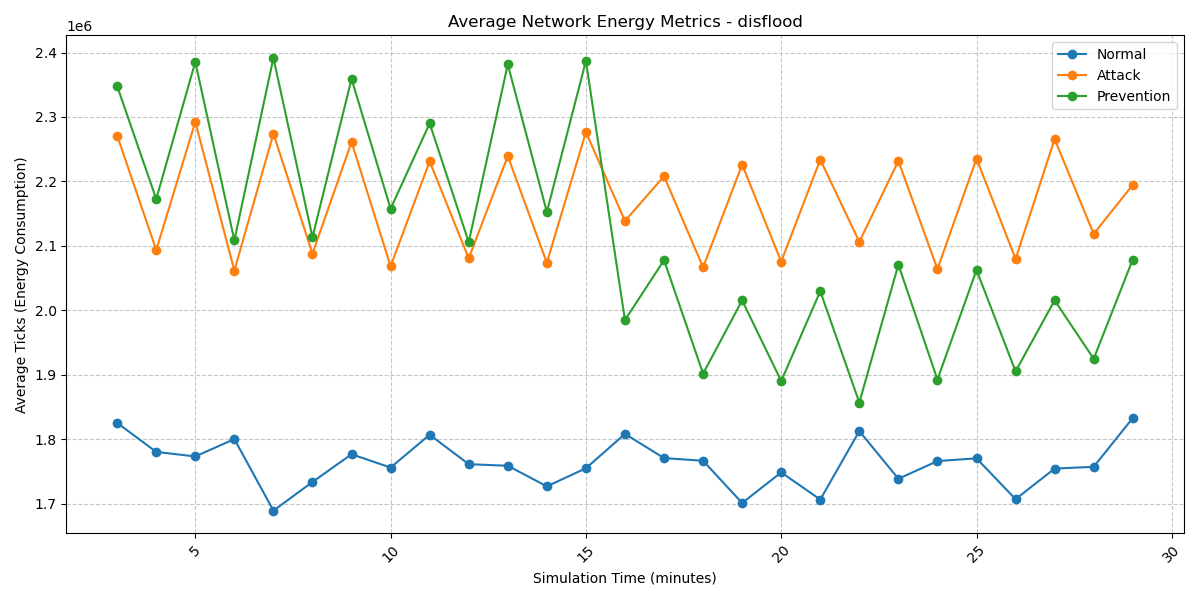
\includegraphics[width=0.48\textwidth]{Figures/energy-usage/energy_plot_disflood_cpu.png}
    \hspace{0.02\textwidth}
    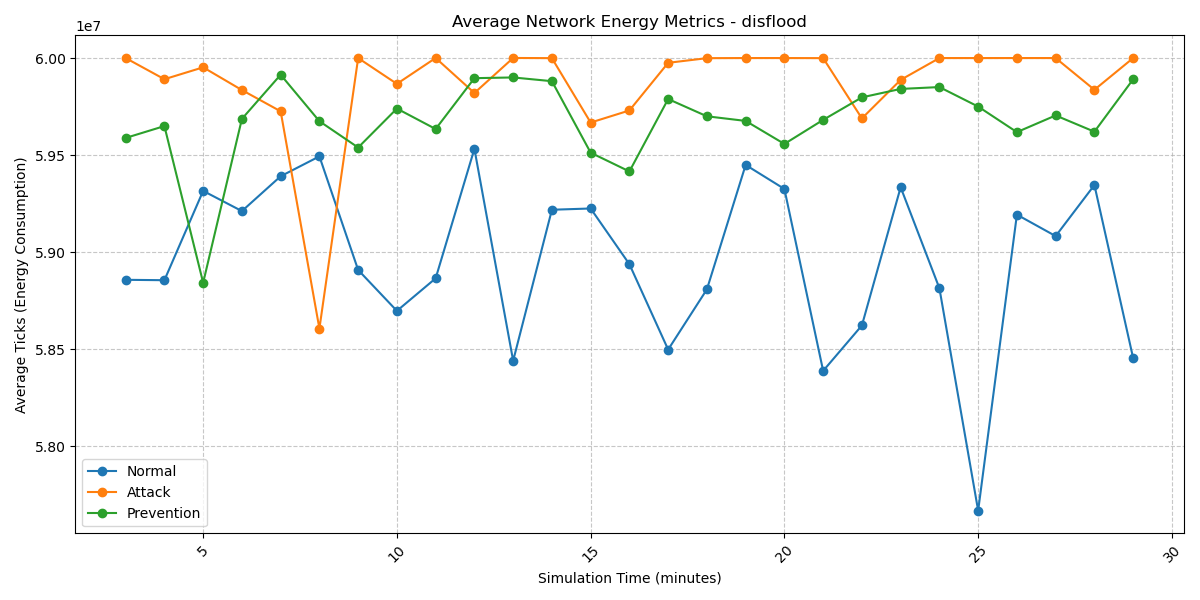
\includegraphics[width=0.48\textwidth]{Figures/energy-usage/energy_plot_disflood_radio_total.png}
    \caption{Tiêu thụ năng lượng DIS Flooding: CPU (trái) và Radio (phải)}
    \label{fig:energy_disflood}
\end{figure}

\subsubsection{DAG Version Attack}
Ngược lại với sự tăng mức tiêu thụ CPU trong kịch bản tấn công DIS, kịch bản tấn công phiên bản lại làm giảm mức tiêu thụ CPU, nhưng lại làm tăng mức tiêu thụ radio. Sự giảm mức tiêu thụ CPU có thể là do việc tấn công phiên bản liên tục khiến các nút bị lỗi phiên bản đồ thị mạng và không thể thực hiện các tác vụ bình thường, dẫn đến việc giảm mức tiêu thụ CPU. Điều tương tự cũng xảy ra với mức tiêu thụ radio. Việc phòng chống nâng mức tiêu thụ CPU từ 1217386 lên 1513039, một khoảng cách đáng kể, và gần với giá trị 1762157 hơn so với khi bị tấn công. Tuy nhiên, nhìn vào đồ thị, lại có thể thấy mức tiêu thụ CPU khi được triển khai biện pháp phòng chống lại có một khoảng tụt xuống gần với mức khi bị tấn công, cụ thể là trong giai đoạn từ 14 đến 26 phút. Với giá trị tiêu thụ Radio, việc phòng chống cho thấy kết quả khả quan hơn, khi đã nâng mức tiêu thụ trung bình từ 56488806 lên 58640745, rất gần với mức bình thường 58959914. Cho thấy phương pháp hash phiên bản đã có hiệu quả trong việc giảm ảnh hưởng đến mức tiêu thụ năng lượng.

Mặc dù một đã có những nghiên cứu cho rằng việc tấn công phiên bản có thể làm tăng mức tiêu thụ năng lượng, kết quả thực nghiệm của nhóm đang cho thấy điều ngược lại. Tuy nhiên, dù mức tiêu thụ năng lượng giảm, ảnh hưởng tiêu cực của tấn công phiên bản, cũng như độ hiệu quả của giải pháp, vẫn rất rõ ràng ở khía cạnh tỉ lệ truyền dữ liệu thành công và chi phí điều khiển RPL.

\begin{figure}[h]
    \centering
    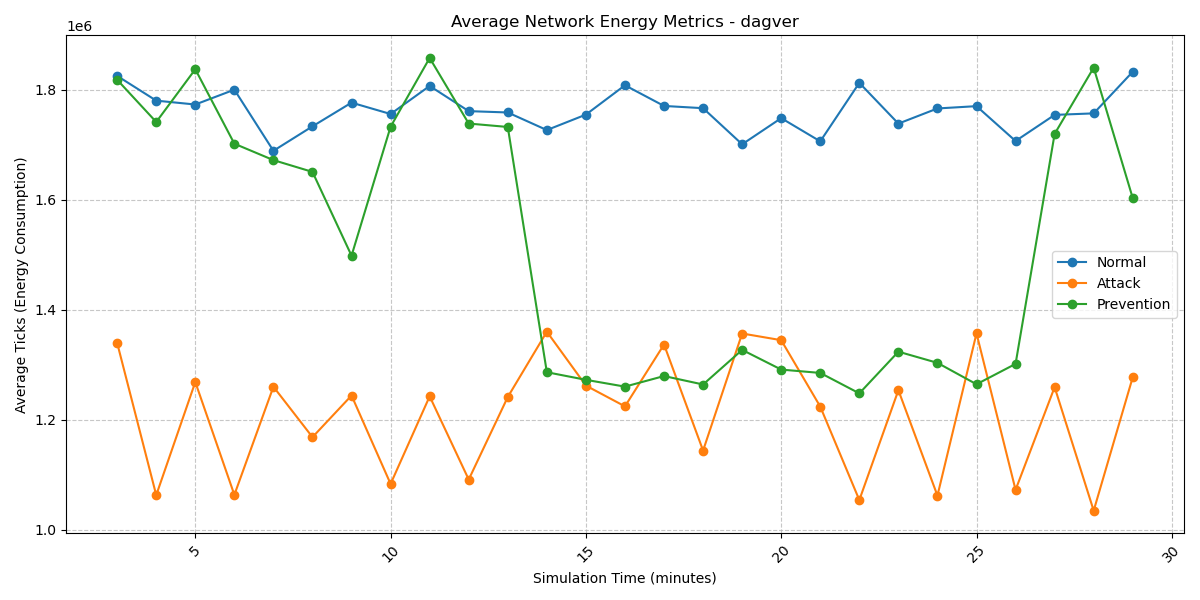
\includegraphics[width=0.48\textwidth]{Figures/energy-usage/energy_plot_dagver_cpu.png}
    \hspace{0.02\textwidth}
    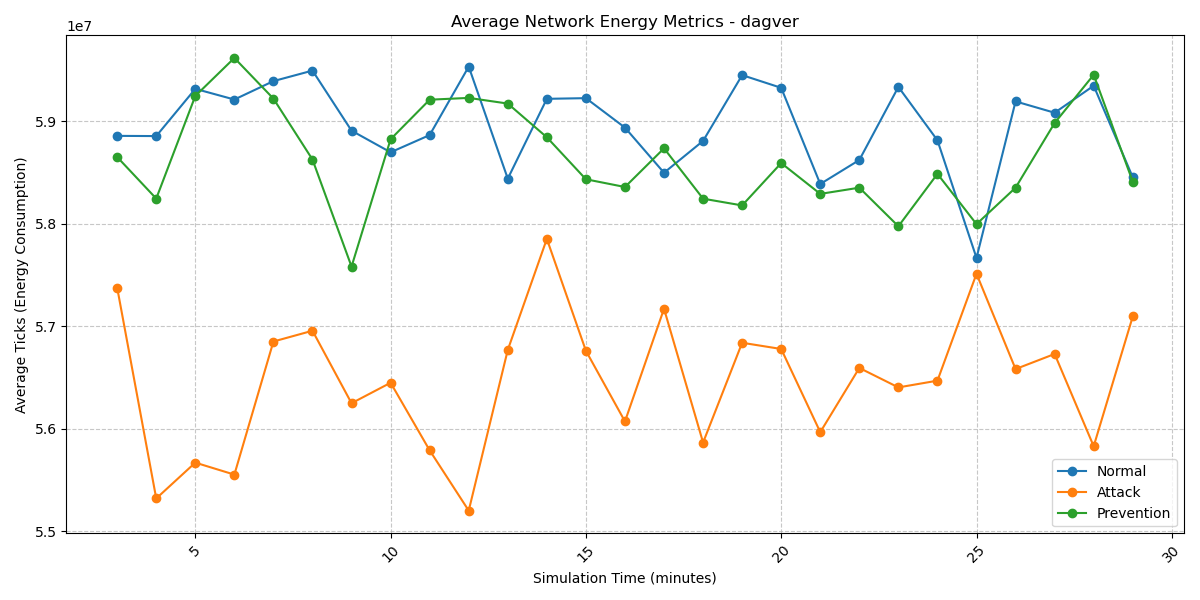
\includegraphics[width=0.48\textwidth]{Figures/energy-usage/energy_plot_dagver_radio_total.png}
    \caption{Tiêu thụ năng lượng DAG Version Attack: CPU (trái) và Radio (phải)}
    \label{fig:energy_dagver}
\end{figure}

\subsubsection{Blackhole Attack}


\begin{figure}[h]
    \centering
    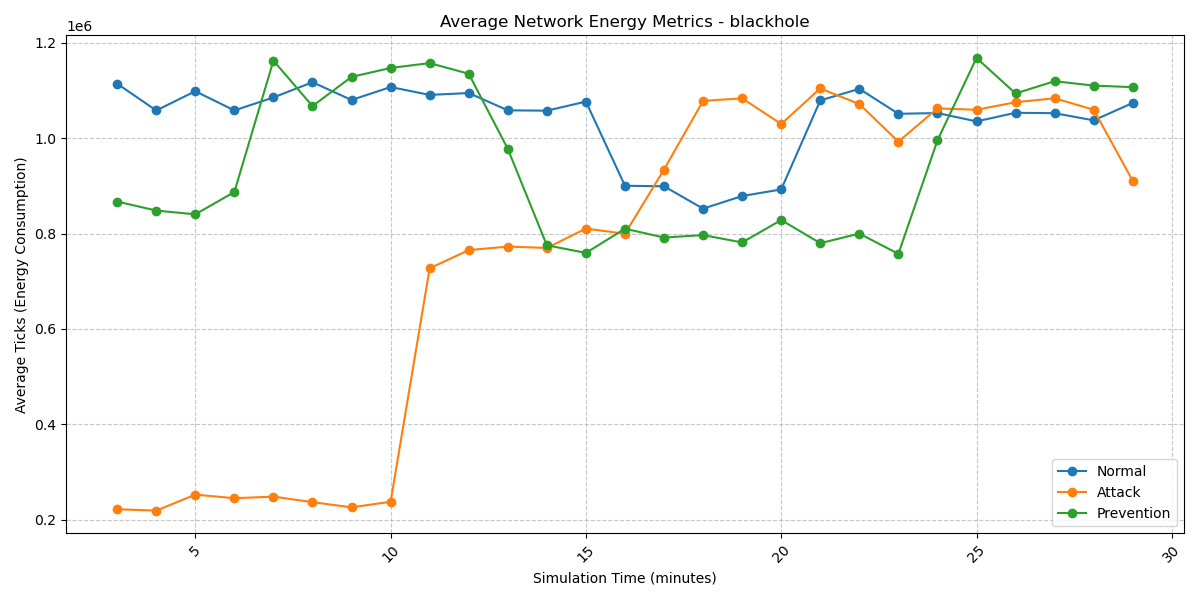
\includegraphics[width=0.48\textwidth]{Figures/energy-usage/energy_plot_blackhole_cpu.png}
    \hspace{0.02\textwidth}
    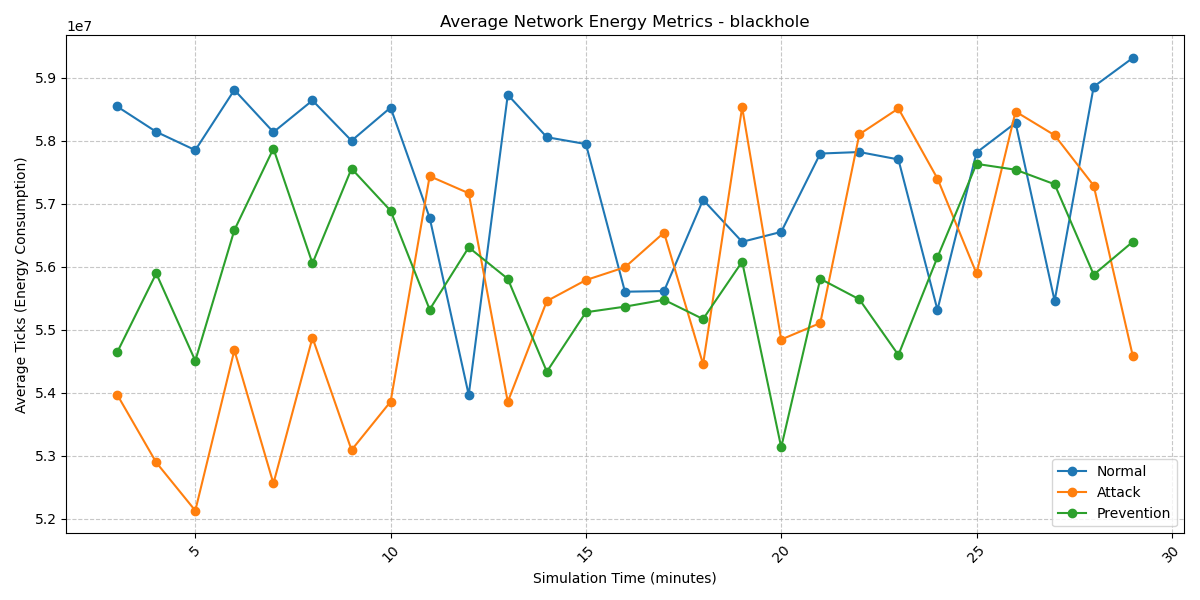
\includegraphics[width=0.48\textwidth]{Figures/energy-usage/energy_plot_blackhole_radio_total.png}
    \caption{Tiêu thụ năng lượng Blackhole Attack: CPU (trái) và Radio (phải)}
    \label{fig:energy_blackhole}
\end{figure}

\subsubsection{Decreased Rank Attack}
Mức tiêu thụ CPU sau khi triển khai biện pháp phòng chống lại tăng gần như đột biến, cho giá trị trung bình 3272003, cao hơn cả giá trị khi bị tấn công (3066664), vốn đã cao hơn gần 2 lần so với mức bình thường (1762156). Mức hoạt động Radio còn cho thấy kết quả khó đánh giá hơn khi liên tục dao động. Giá trị hoạt động trung bình của radio (59446677 chu kỳ/phút) sau khi triển khai biện pháp phòng chống lại còn cao hơn so với khi bị tấn công (59297215 chu kỳ/phút), và cả hai đều cao hơn so với mức bình thường (58959914 chu kỳ/phút). Như vậy, biện pháp phòng chống đã không có hiệu quả trong việc giảm mức tiêu thụ năng lượng, mà thậm chí còn làm tăng mức tiêu thụ năng lượng lên đáng kể.

\begin{figure}[h]
    \centering
    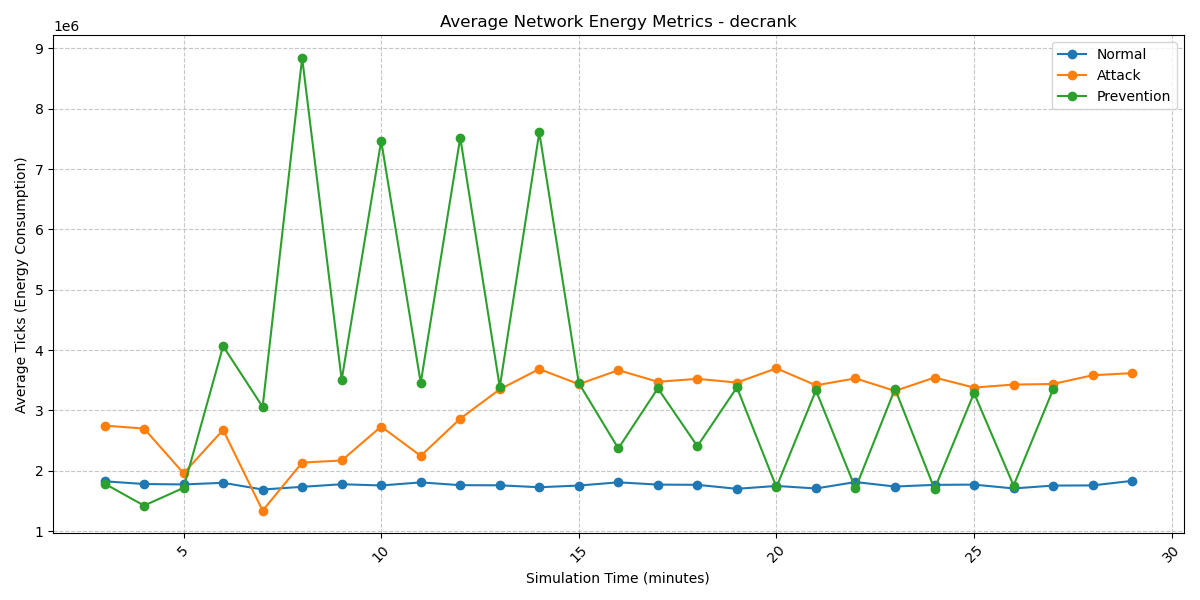
\includegraphics[width=0.48\textwidth]{Figures/energy-usage/energy_plot_decrank_cpu.png}
    \hspace{0.02\textwidth}
    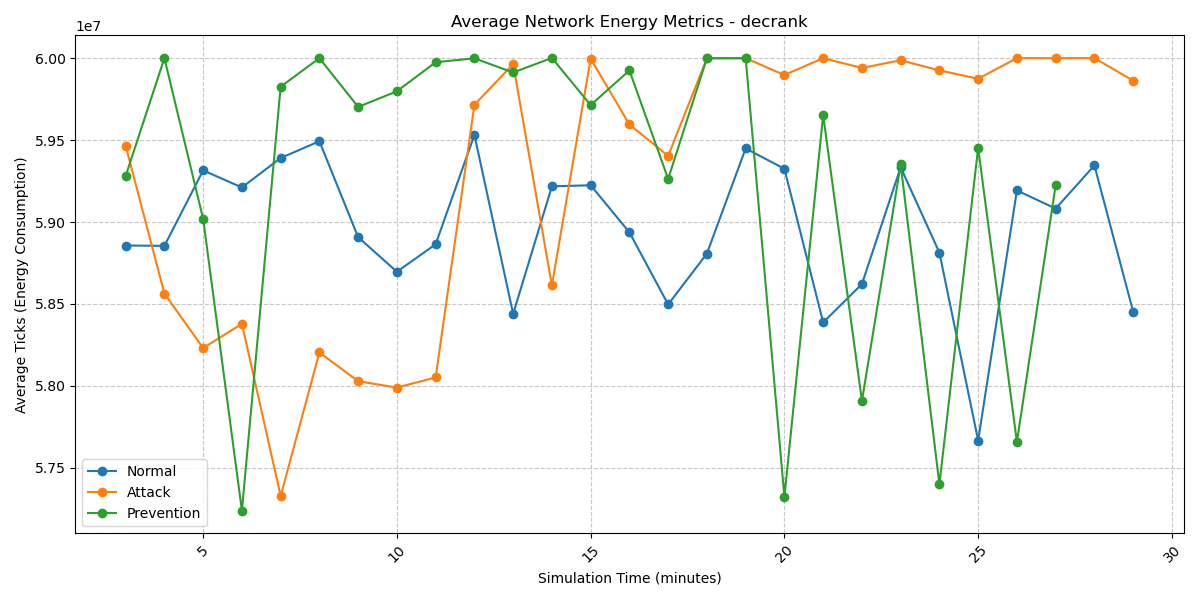
\includegraphics[width=0.48\textwidth]{Figures/energy-usage/energy_plot_decrank_radio_total.png}
    \caption{Tiêu thụ năng lượng Decreased Rank Attack: CPU (trái) và Radio (phải)}
    \label{fig:energy_decrank}
\end{figure}

\subsection{Tổng kết}
Trong chương này, nhóm đã trình bày quá trình thực nghiệm và kết quả đánh giá thu được từ quá trình đó. Các biện pháp phòng chống nhìn chung đã có tác động tích cực đến một số chỉ số (tỉ lệ truyền thành công, chi phí gói tin điều khiển), nhưng lại chưa đủ hiệu quả trong việc giảm mức tiêu thụ năng lượng, thậm chí còn làm tăng mức tiêu thụ năng lượng lên đáng kể trong một số kịch bản. Với thời gian thực nghiệm hạn chế, nhóm chưa thể xác định được nguyên nhân là do bản thân biện pháp phòng chống hay do hướng tiếp cận của nhóm trong việc hiện thực hoá chưa chuẩn xác.
\newpage
% ============================================================
%  Chapter 6.tex — KẾT LUẬN VÀ HƯỚNG PHÁT TRIỂN
% ============================================================
\section{KẾT LUẬN VÀ HƯỚNG PHÁT TRIỂN}
\label{sec:ch6}

% TODO: Nội dung chương 6.

\newpage

% ---------- Tài liệu tham khảo ----------
\phantomsection
\addcontentsline{toc}{section}{\numberline{}TÀI LIỆU THAM KHẢO}
\nocite{*}
\bibliographystyle{IEEEtran}
\bibliography{References}

% ---------- Phụ lục ----------
\newpage
% ============================================================
%  Appendix.tex — Phụ lục
% ============================================================
\section*{PHỤ LỤC}
\phantomsection
\addcontentsline{toc}{section}{\numberline{}PHỤ LỤC}
\setcounter{section}{0}
\renewcommand{\thesection}{\Alph{section}}

% ============================================================
\section{Mã nguồn IDS (Contiki-NG)}
\label{app:code}
% ============================================================

\subsection{Module phát hiện DIS Flooding}

% TODO: dán mã nguồn C vào đây, ví dụ:
% \lstinputlisting[language=C,
%   caption={ids\_dis\_flooding.c}]{Code/ids_dis_flooding.c}

\begin{lstlisting}[language=C, caption={Skeleton: ids\_dis\_flooding.c}]
#include "contiki.h"
#include "net/routing/rpl-lite/rpl.h"

/* Nguong so ban tin DIS trong mot chu ky Trickle */
#define DIS_FLOOD_THRESHOLD  10

static uint16_t dis_count = 0;

void ids_dis_on_receive(void) {
  dis_count++;
  if (dis_count > DIS_FLOOD_THRESHOLD) {
    /* TODO: Kich hoat canh bao DIS Flooding */
  }
}
\end{lstlisting}

\subsection{Module phát hiện Blackhole}

\begin{lstlisting}[language=C, caption={Skeleton: ids\_blackhole.c}]
#include "contiki.h"

#define PDR_THRESHOLD  0.7   /* PDR duoi 70% -> nghi ngo Blackhole */

float ids_compute_pdr(uint16_t sent, uint16_t received) {
  if (sent == 0) return 1.0f;
  return (float)received / (float)sent;
}
\end{lstlisting}

\subsection{Module phát hiện Decreased Rank}

\begin{lstlisting}[language=C, caption={Skeleton: ids\_decreased\_rank.c}]
#include "contiki.h"
#include "net/routing/rpl-lite/rpl.h"

void ids_rank_check(rpl_dag_t *dag, rpl_parent_t *parent,
                    rpl_rank_t advertised_rank) {
  rpl_rank_t expected = /* tinh toan rank du kien */ 0;
  if (advertised_rank < expected) {
    /* TODO: Danh dau parent nay la nghi ngo */
  }
}
\end{lstlisting}

\subsection{Module phát hiện VeRA / Version Number Attack}

\begin{lstlisting}[language=C, caption={Skeleton: ids\_vera.c}]
#include "contiki.h"
#include "net/routing/rpl-lite/rpl.h"

static uint8_t last_known_version = 0;

void ids_version_check(uint8_t received_version) {
  if (received_version > last_known_version + 1) {
    /* TODO: Version tang bat thuong -> canh bao VeRA attack */
  }
  last_known_version = received_version;
}
\end{lstlisting}

% ============================================================
\section{Cấu hình mô phỏng Cooja}
\label{app:cooja}
% ============================================================

\subsection{Tham số mô phỏng}

\begin{table}[H]
\centering
\caption{Tham số cấu hình chung trong Cooja}
\begin{tabularx}{\textwidth}{lX}
  \toprule
  \textbf{Tham số} & \textbf{Giá trị} \\
  \midrule
  Mô phỏng radio    & Unit Disk Graph Medium (UDGM) \\
  Số nút tổng       & 20 nút (1 Border Router + 19 mote) \\
  Tỉ lệ nút tấn công & 0\%, 10\%, 25\%, 50\% \\
  Thời gian mô phỏng & 300 giây / kịch bản \\
  Tần suất gửi dữ liệu & 1 gói / 10 giây \\
  Hệ điều hành      & Contiki-NG 4.x \\
  Objective Function & MRHOF (ETX metric) \\
  \bottomrule
\end{tabularx}
\end{table}

\subsection{Hướng dẫn chạy mô phỏng}

\begin{enumerate}
  \item Cài đặt Contiki-NG và Cooja theo hướng dẫn tại
        \url{https://github.com/contiki-ng/contiki-ng/wiki}.
  \item Mở file \texttt{simulation/rpl\_ids\_scenario.csc} trong Cooja.
  \item Chọn kịch bản tấn công trong menu \textbf{Simulation Parameters}.
  \item Nhấn \textbf{Start} và quan sát log từ \textbf{Mote Output}.
  \item Xuất kết quả ra file \texttt{.csv} để phân tích với script Python
        trong thư mục \texttt{analysis/}.
\end{enumerate}


\end{document}
